\documentclass[compress]{beamer}
\mode<presentation>
\usetheme{Warsaw}
\usecolortheme{seagull}
%\useoutertheme[subsection=false]{smoothbars}
\useoutertheme{infolines}
\useinnertheme{rectangles}

\setbeamercovered{dynamic}

\usepackage{array}
\usepackage{amsmath,amssymb,amsfonts,mathrsfs,amsthm}
\usepackage[utf8]{inputenc}
\usepackage{listings}
\usepackage{mathtools}
\usepackage{dsfont}
\usepackage{pdfpages}
\usepackage[textsize=footnotesize,color=green]{todonotes}
\usepackage{algorithm, algorithmic}
\usepackage{bm}
\usepackage{tikz}
\usepackage[normalem]{ulem}

\usepackage{graphicx}
\usepackage{subfigure}
%\usepackage{caption}
%\usepackage{subcaption}

\usepackage{color}
\usepackage{undertilde}
\usepackage{pdflscape}
\usepackage{pifont}

\usepackage{bibentry}
\nobibliography*

%\usepackage[osf]{mathpazo}
%\usepackage{mathpazo}
%\renewcommand\rmdefault{ptm}

\renewcommand{\topfraction}{0.85}
\renewcommand{\textfraction}{0.1}
\renewcommand{\floatpagefraction}{0.75}

\newcommand{\vect}[1]{\ensuremath\boldsymbol{#1}}
\newcommand{\tensor}[1]{\underline{\vect{#1}}}
\newcommand{\del}{\triangle}
\newcommand{\grad}{\nabla}
\newcommand{\curl}{\grad \times}
\renewcommand{\div}{\grad \cdot}
\newcommand{\ip}[1]{\left\langle #1 \right\rangle}
\newcommand{\eip}[1]{a\left( #1 \right)}
\newcommand{\pd}[2]{\frac{\partial#1}{\partial#2}}
\newcommand{\pdd}[2]{\frac{\partial^2#1}{\partial#2^2}}

\newcommand{\circone}{\ding{192}}
\newcommand{\circtwo}{\ding{193}}
\newcommand{\circthree}{\ding{194}}
\newcommand{\circfour}{\ding{195}}
\newcommand{\circfive}{\ding{196}}

\newcommand{\Reyn}{\rm Re}

\newcommand{\bs}[1]{\boldsymbol{#1}}
\DeclareMathOperator{\diag}{diag}

\newcommand{\equaldef}{\stackrel{\mathrm{def}}{=}}

\newcommand{\tablab}[1]{\label{tab:#1}}
\newcommand{\tabref}[1]{Table~\ref{tab:#1}}

\newcommand{\theolab}[1]{\label{theo:#1}}
\newcommand{\theoref}[1]{\ref{theo:#1}}
\newcommand{\eqnlab}[1]{\label{eq:#1}}
\newcommand{\eqnref}[1]{\eqref{eq:#1}}
\newcommand{\seclab}[1]{\label{sec:#1}}
\newcommand{\secref}[1]{\ref{sec:#1}}
\newcommand{\lemlab}[1]{\label{lem:#1}}
\newcommand{\lemref}[1]{\ref{lem:#1}}

\newcommand{\mb}[1]{\mathbf{#1}}
\newcommand{\mbb}[1]{\mathbb{#1}}
\newcommand{\mc}[1]{\mathcal{#1}}
\newcommand{\nor}[1]{\left\| #1 \right\|}
\newcommand{\snor}[1]{\left| #1 \right|}
\newcommand{\LRp}[1]{\left( #1 \right)}
\newcommand{\LRs}[1]{\left[ #1 \right]}
\newcommand{\LRa}[1]{\left\langle #1 \right\rangle}
\newcommand{\LRc}[1]{\left\{ #1 \right\}}
\newcommand{\tanbui}[2]{\textcolor{blue}{\sout{#1}} \textcolor{red}{#2}}
\newcommand{\Grad} {\ensuremath{\nabla}}
\newcommand{\Div} {\ensuremath{\nabla\cdot}}
\newcommand{\Nel} {\ensuremath{{N^\text{el}}}}
\newcommand{\jump}[1] {\ensuremath{\LRs{\![#1]\!}}}
\newcommand{\uh}{\widehat{u}}
\newcommand{\fnh}{\widehat{f}_n}
\renewcommand{\L}{L^2\LRp{\Omega}}
\newcommand{\pO}{\partial\Omega}
\newcommand{\Gh}{\Gamma_h}
\newcommand{\Gm}{\Gamma_{-}}
\newcommand{\Gp}{\Gamma_{+}}
\newcommand{\Go}{\Gamma_0}
\newcommand{\Oh}{\Omega_h}

\newcommand{\eval}[2][\right]{\relax
  \ifx#1\right\relax \left.\fi#2#1\rvert}

\def\etal{{\it et al.~}}


\def\arr#1#2#3#4{\left[
\begin{array}{cc}
#1 & #2\\
#3 & #4\\
\end{array}
\right]}
\def\vecttwo#1#2{\left[
\begin{array}{c}
#1\\
#2\\
\end{array}
\right]}
\def\vectthree#1#2#3{\left[
\begin{array}{c}
#1\\
#2\\
#3\\
\end{array}
\right]}
\def\vectfour#1#2#3#4{\left[
\begin{array}{c}
#1\\
#2\\
#3\\
#4\\
\end{array}
\right]}

\newcommand{\G} {\Gamma}
\newcommand{\Gin} {\Gamma_{in}}
\newcommand{\Gout} {\Gamma_{out}}

% removes nav symbols
\beamertemplatenavigationsymbolsempty

% defines newblock as null, giving compile issues otherwise
\let\newblock\relax 

\institute[ICES]{Institute for Computational Engineering and Sciences}

\title[A DPG method for Compressible Flow]{A Discontinuous Petrov-Galerkin method for compressible flow problems}
\date{August 15, 2012}
\author[J. Chan, T. Ellis, L. Demkowicz, R. Moser]{Jesse Chan, Truman Ellis \\ Supervisors: Leszek Demkowicz, Robert Moser}

\begin{document}
\begin{frame}
\maketitle
\end{frame}

\frame{
\frametitle{Compressible Navier-Stokes equations}
\begin{columns}[c]
\begin{column}{.475\textwidth}
Numerical difficulties:
\begin{itemize}
\item{} Resolving solution features (sharp, localized viscous-scale phenomena)
\begin{itemize}
\item{} Shocks
\item{} Boundary layers - resolution needed for drag/load
\item{} Turbulence (non-localized)
\end{itemize}
\item{} Nonlinear convergence and uniqueness of solutions
\item{} Stability of numerical schemes
\begin{itemize}
\item{} Coarse/adaptive grids
\item{} Higher order
\end{itemize}
\end{itemize}
\end{column}
\begin{column}{.475\textwidth}
\begin{figure}
\centering
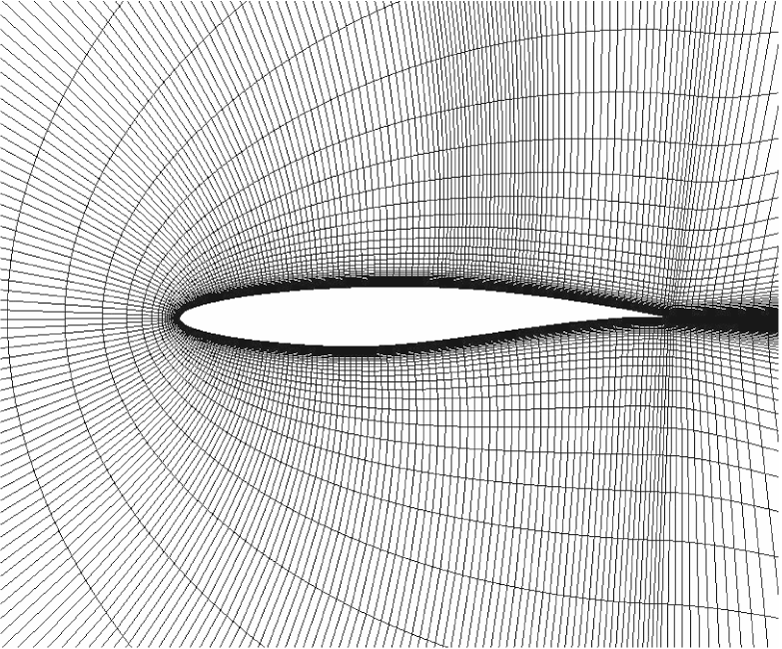
\includegraphics[scale = .7]{figs/compFlowPics/airfoil_mesh.png}
\end{figure}
\end{column}
\end{columns}
\vspace{.2cm}
\begin{center}
Idea: begin first with the model problem of convection-diffusion.
\end{center}
}
\frame{
\frametitle{Robustness: convection-diffusion as a model problem}
\vspace{-.5cm}
\[
\div \left(\beta u\right) - \epsilon \Delta u = f, \quad \text{on }\Omega \in \mathbb{R}^3
\]
\vspace{-.5cm}
\begin{columns}[c]
\begin{column}{.49\textwidth}
In 1D: $\beta u' - \epsilon u'' = f$. Standard continuous Galerkin variational formulation: solve
\[
b(u,v) = \ell(v), \quad u,v\in H^1_0([0,1])
\]
where
\begin{align*}
b(u,v) &= \int_\Omega -\beta uv' + \epsilon u'v' \\
\ell(v) &= \int_\Omega f v 
\end{align*}
\end{column}
\begin{column}{.49\textwidth}
\begin{figure}
\centering
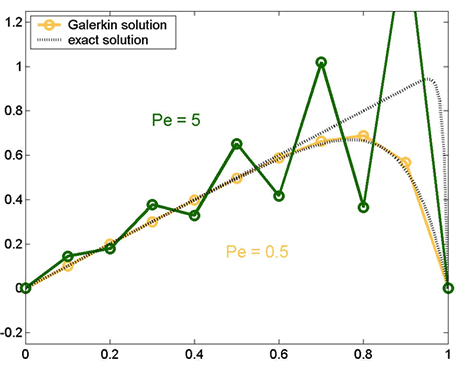
\includegraphics[scale=.35]{figs/GalerkinOscTight.png}
\caption{Solution for $f=1$. Oscillations in the standard Galerkin method for large Peclet numbers ${\rm Pe} \coloneqq \frac{h}{\epsilon}$.}
\end{figure}
\end{column}
\end{columns}
}

\frame{
\frametitle{Streamline-upwind Petrov-Galerkin (SUPG)}
SUPG solves $b_{\rm SUPG}(u,v) = l_{\rm SUPG}(v)$, where
\begin{align*}
b_{\rm SUPG}(u,v) &= b(u,v)+ \sum_{K} \int_{K} \tau \LRp{L_{\rm adv} v} L u \\
l_{\rm SUPG}(v) &= \ell(v) + \sum_{K} \int_{K} \tau \LRp{L_{\rm adv}v} f.
\end{align*}
\vspace{-.5cm}
\begin{columns}[c]
\begin{column}{.44\textwidth}
\vspace{-.5cm}
\begin{itemize}
\item{} $Lu = \div\left(\beta u\right) - \epsilon \triangle u$, $L_{\rm adv}u = \div \left(\beta u\right)$, and $\tau$ is a parameter. 
%\item{} Recovers ``exact'' artificial diffusion for $f=0$.
\item{} Effective for $f\neq 0$. %``exact'' artificial diffusion.
\item{} \emph{Residual-based} stabilization. 
\end{itemize}
\end{column}
\begin{column}{.54\textwidth}
\begin{figure}
\centering
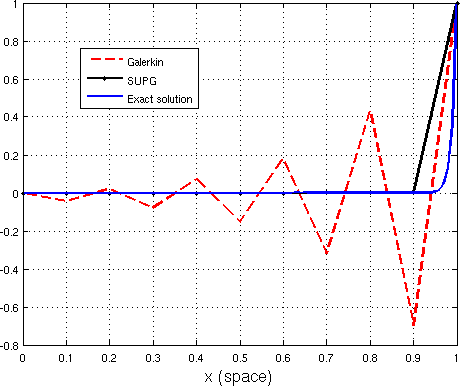
\includegraphics[scale=.38]{figs/SUPG.png}
%\caption{Exact, Bubnov-Galerkin, and SUPG solutions.}
\end{figure}
\end{column}
\end{columns}
}

\frame{
\begin{columns}
\begin{column}{.49\textwidth}
Can be interpreted as a \emph{Petrov-Galerkin} method,
\[
b\LRp{u,\tilde{v}_{i}} = \ell\LRp{\tilde{v}_{i}}, \quad \forall i = 1,\ldots,N-1,
\]
where the SUPG test function $\tilde{v}_{i}$ is defined elementwise as\footnotemark
\[
\tilde{v}_{i} = \phi_i(x) + \tau L_{\rm adv} \phi_i.  
\]
\end{column}
\begin{column}{.49\textwidth}
\begin{figure}
\centering
\subfigure{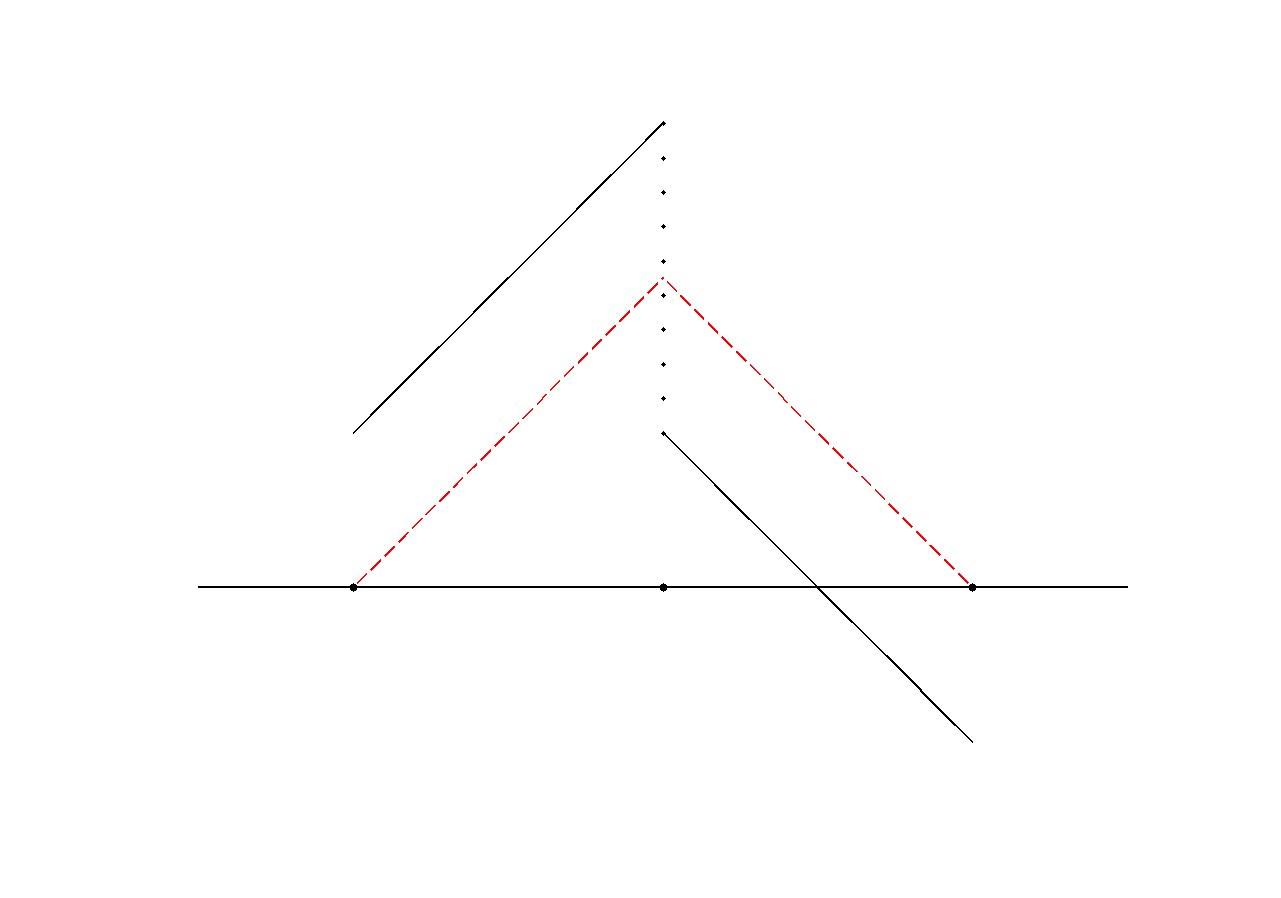
\includegraphics[scale=.16]{figs/SUPGtest.png}}
\caption{SUPG test function $v_i$.}
\end{figure}
\end{column}
\end{columns}
\footnotetext{\bibentry{SUPG}}
}

\section{The DPG Method}
\frame{
\frametitle{DPG: a minimum residual method via optimal testing}
Given a trial space $U$ and Hilbert test space $V$,
\[
b(u,v) = \ell(v), \quad u\in U, \quad v\in V
\]
This is equivalent to the operator equation posed in $V'$
\[
Bu = \ell
\]
if we identify $B:U\rightarrow V'$ and $\ell\in V'$ such that 
\begin{align*}
\langle Bu,v\rangle_V &\coloneqq b(u,v), \quad u\in U, v\in V,\\
\langle \ell,v\rangle_V &\coloneqq \ell(v), \quad v\in V.
\end{align*}
We seek to minimize the dual functional over $U_h \subset U$
\[
J(u_h) = \frac{1}{2}\|Bu_h-\ell\|_{V'}^2 \coloneqq\frac{1}{2} \sup_{v\in V\setminus\{0\}} \frac{| b(u_h,v)-\ell(v)|^2}{\nor{v}_V^2}.
\]
}

\begin{frame}
Let $R_V: V \to V'$ be the isometric Riesz map st.\
\[
\langle R_V v,\delta v\rangle_V \coloneqq(v, \delta v)_V, \quad \forall \delta v \in V.
\]
Then, our functional $J(u_h)$ is equal to
\begin{equation*}
\min_{u_h\in U_h} J(u_h) = \frac{1}{2}\left\|Bu_h-\ell\right\|_{V'}^2 =  \frac{1}{2}\left\|R_V^{-1}(Bu_h-\ell)\right\|_V^2.
\end{equation*}
First order optimality: G\^ateaux derivative is zero in all directions $\delta u \in U_h$
\begin{align*}
\left(R_V^{-1}(Bu_h-\ell),R_V^{-1}B\delta u\right)_V &= 0, \quad \forall \delta u \in U_h.\\
\rightarrow \LRa{(Bu_h-\ell),R_V^{-1}B\delta u} &= 0, \\
\rightarrow b(u_h,R_V^{-1}B\delta u) - \ell(R_V^{-1}B\delta u) &= 0
\end{align*}
\end{frame}

\frame{
\frametitle{Summary: select test functions to minimize residuals}
For $\delta u \in U_h$, define the \textcolor{red}{optimal test function} $v_{\delta u}$. 
\begin{equation*}
v_{\delta u} \coloneqq R_V^{-1}B\delta u.
\end{equation*} 
Then, the residual $J(u_h) = \frac{1}{2}\left\|Bu_h-\ell\right\|_{V'}^2$ is minimized by the solution of
\[
b\LRp{u_h,v_{\delta u}} = \ell\LRp{v_{\delta u}}, \quad \forall \delta u \in U_h.
\]
}

\frame{
\frametitle{Practical details of DPG}
Computation of $v_{\delta u} \coloneqq R_V^{-1}B\delta u$ is \textbf{global} and \textbf{infinite-dimensional}.
\begin{itemize}
\item By choosing a \textcolor{red}{broken} test space $V$ and \textcolor{red}{localizable} norm $\nor{v}_V^2 = \sum_K \nor{v}_{V(K)}^2$, test functions can be determined locally.
\item In practice, we use an \textcolor{red}{enriched space} $V_h \subset V$, where $\dim(V_h) > \dim(U_h)$ elementwise, and \textcolor{red}{optimal test functions} are approximated by computing $v_{\delta u} \coloneqq R_{V_h}^{-1}B\delta u \in V_h$ through\footnote{\bibentry{DPG2}}
\[
\LRp{v_{\delta u},\delta v}_V = b(\delta u,\delta v), \quad \delta u\in U_h, \quad \forall \delta v\in V_h
\]
Typically, if $U_h = \mathcal{P}^p(\mathbb{R}^n)$, $V_h = \mathcal{P}^{p+\triangle p}(\mathbb{R}^n)$, where $\triangle p \geq n$.\footnote{\bibentry{practicalDPG}} 
\end{itemize}
%\footnotetext{\bibentry{DPG2}}
}

\frame{
\frametitle{Properties of DPG}
DPG provides a symmetric positive-definite stiffness matrix. Let $\{\phi_j\}_{j=1}^m$ be a basis for $U_h$, and $\{v_i\}_{i=1}^n$ a basis for $V_h$, such that $n>m$. Then, for 
\begin{align*}
B_{ji} &= b(\phi_j,v_i),\\
l_i &= \ell(v_i),
\end{align*}
DPG solves the discrete system for degrees of freedom $u$
\begin{align*}
\LRp{B^T R_V^{-1}B} u  &= \LRp{B^T R_V^{-1}} l,
\end{align*}
where, under a localizable norm and discontinuous test functions, $R_V^{-1}$ is block diagonal.
}

\frame{
\frametitle{Properties of DPG}
Additional properties of DPG include\footnotemark
\begin{itemize}
\item DPG provides the best approximation in the \textcolor{red}{energy norm}
\[
\|u\|_E = \|Bu\|_{V'} = \sup_{\nor{v}_V=1} \left|b(u,v)\right|.
\]
\item The energy error is computable through the residual
\[
\nor{u-u_h}_E = \nor{B(u-u_h)}_{V'} = \nor{R_V^{-1}(l-Bu_h)}_V = \nor{e}_V
\]
where the \textcolor{red}{error representation function} $e$ is defined through $(e,\delta v)_V = \ell(v)-b(u_h,\delta v)$ for all $\delta v\in V$. 
\end{itemize}
\footnotetext{\bibentry{DPG3pub}}
}

%\frame{
%\frametitle{Duality of norms}
%Duality of norms: for any trial norm $\nor{u}_U$,
%\[
%\nor{u}_{U} = \sup_{v \in V}\frac{b\LRp{u,v}}{\nor{v}_{V,U}}, \quad \nor{v}_{V,U} = \sup_{u \in U}\frac%{b\LRp{u,v}}{\nor{u}_{U}}.
%\]
%Likewise, for any test norm $\nor{v}_V$, 
%\[
%\nor{v}_{V} = \sup_{u \in U}\frac{b\LRp{u,v}}{\nor{U}_{U,V}}, \quad \nor{u}_{U,V} = \sup_{v \in V}\frac%{b\LRp{u,v}}{\nor{v}_{V}}.
%\]
%
%}

\frame{
\frametitle{Ultra-weak formulation}
\vspace{-.75cm}
\begin{columns}
\begin{column}{.64\textwidth}
Given a first order system $Au = f$, we identify the \textbf{\emph{partition}} $\Oh$ and \textbf{\textcolor{red}{mesh skeleton}} \textcolor{red}{$\Gh$}.
\end{column}
\begin{column}{.34\textwidth}
%\[
%\Oh = \cup_{j=1}^\Nel K_j, \quad \Gh = \cup_{j=1}^\Nel \partial K_j
%\]
\begin{figure}[!h]
\centering
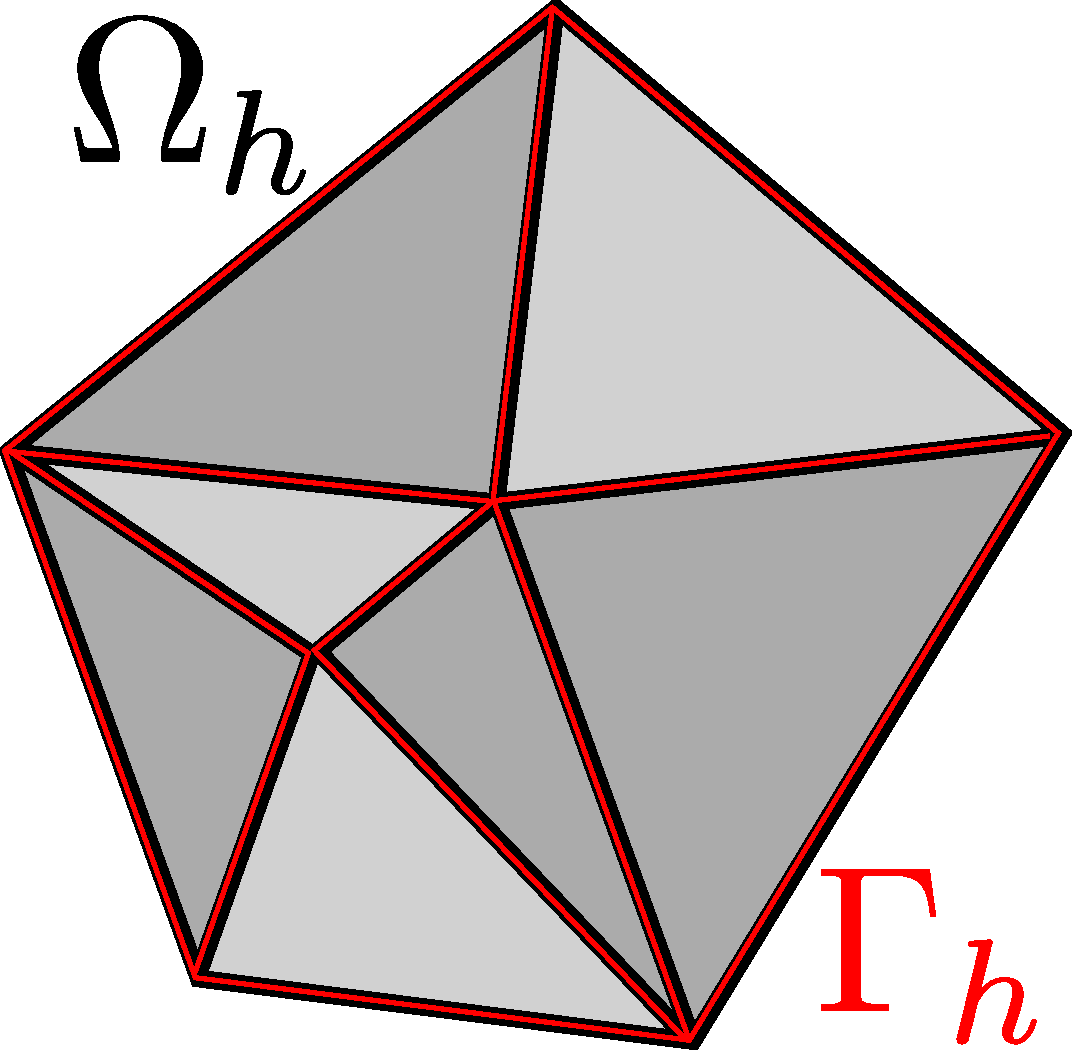
\includegraphics[scale = .155]{mesh_skel.pdf}
\end{figure}
\end{column}
\end{columns}
\vspace{-.5cm}
The ultra-weak formulation for $Au = f$ on $\Oh$ is
\[
b\left(\left(u, \widehat{u}\right),v\right) \coloneqq \sum_K\langle \widehat{u},v \rangle_{\partial K} + (u,A_h^*v)_{\Oh}= \LRp{f,v}_{\Oh}.
\]
Under proper assumptions, $\sum_K\langle \widehat{u},v \rangle_{\partial K} = \langle \widehat{u}, \jump{v} \rangle_{\Gh}$, with energy setting
\[
u\in L^2\LRp{\Oh} \equiv L^2(\Omega), \quad v\in V=D(A^*_h), \quad
\widehat{u}\in \gamma(D(A)),
\]
where $D(A_h^*)$ is the broken graph space of the formal adjoint $A_h^*$, and $\gamma(D(A))$ the trace space of the graph space of operator $A$.\footnote{\bibentry{analysisDPG}}
}

\frame{
\frametitle{The canonical ``graph'' test norm}
Recall $\nor{u}_E \coloneqq \sup_{v\in V\setminus\{0\}}\frac{b(u,v)}{\nor{v}_V}$. Under the ultra-weak formulation, the trial norm 
\[
\nor{\LRp{u,\widehat{u}}}_U \coloneqq \|u\|^2_{\L} + \|\widehat{u}\|^2
\] 
generates a test norm \emph{equivalent} to 
\[
\nor{v}_{V_{\rm opt}} \coloneqq \|A_h^*v\|_{\L}^2 +\left(\sup_{\widehat{u}} \frac{\LRa{ \widehat{u},\jump{v} }_{\Gh}}{\|\widehat{u}\|}\right)^2.
\]
This norm is not localizable, so we instead substitute the jump terms for an $L^2$ term, giving us the \emph{graph norm}\footnote{\bibentry{Bui-ThanhDemkowiczGhattas11b}}
\[
\nor{v}_V \coloneqq \|A_h^*v\|_{\L}^2 + \nor{v}_{L^2}.
\]
}

\frame{
\frametitle{Goal: robust higher order adaptive methods}
\begin{columns}
\begin{column}{.45\textwidth}
Our aim is to design an adaptive method for compressible laminar flows that is 
\begin{itemize}
\item robust in Reynolds number
\item stable for arbitrary elements
\end{itemize}

This proposal will outline
\begin{enumerate}
\item a robust DPG method for convection-diffusion,
\item extension to nonlinear problems and systems,
\item proposed work.
\end{enumerate}

\end{column}
\begin{column}{.54\textwidth}
\begin{figure}
\centering
\subfigure{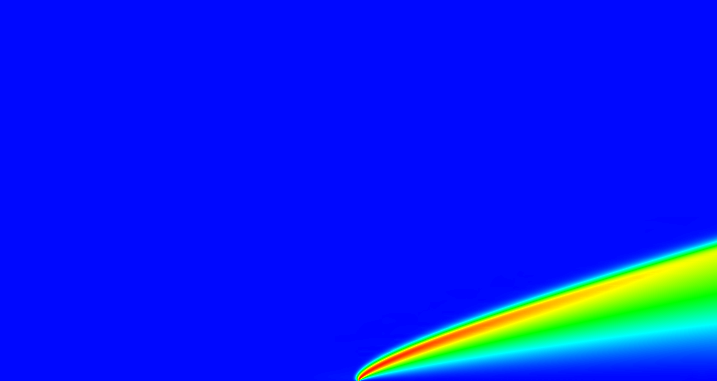
\includegraphics[scale=.23]{figs/Re1000p2/u2_full.png}}
\subfigure{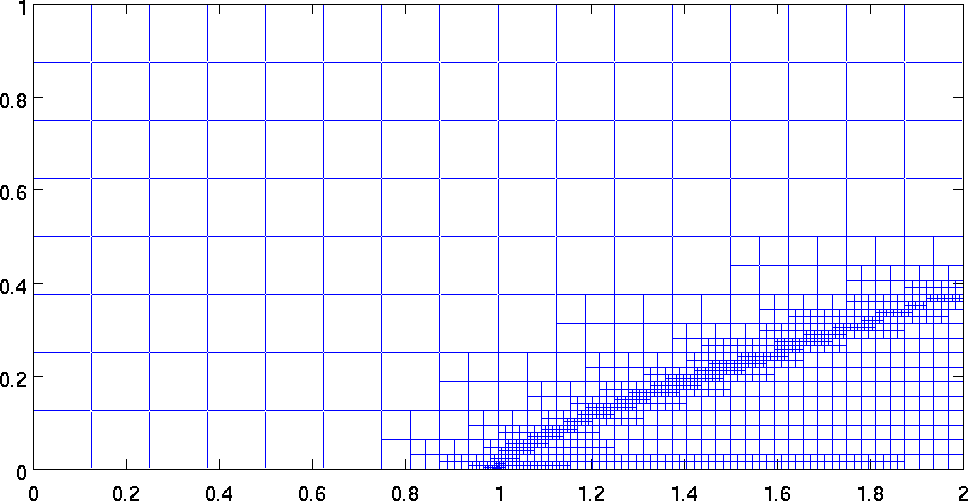
\includegraphics[scale=.37]{figs/Re1000p2/mesh6.png}}
\caption{$u_2$ and $p=2$ mesh for $\Reyn = 1000$.}
\end{figure}
\end{column}
\end{columns}
}

\section{A Robust DPG Method for Convection-Diffusion}

\frame{
\frametitle{Ultra-weak formulation for convection-diffusion}
In first order form, the convection-diffusion equation is
\[
A \LRp{u,\sigma} \coloneqq 
\LRs {
\begin{array}{c}
\div (\beta u - \sigma) \\ \frac{1}{\epsilon}\sigma - \grad u
\end{array}} = \LRs{
\begin{array}{c}
f \\ 0
\end{array}
}.
\]
The variational formulation is
\begin{align*}
b\left(\left(u,\sigma, \widehat{u}, \widehat{f}_n\right),
\left( v, \tau \right)\right) = \left(u,\grad_h\cdot \tau - \beta \cdot \grad_h
v\right)_{\Oh} + \left(\sigma, \epsilon^{-1} \tau + \grad_h v\right)_{\Oh}&\\
  - \LRa{\jump{\tau\cdot n}, \widehat{u} }_{\Gh} + \LRa{\widehat{f}_n,\jump{v} }_{\Gh}&,
\end{align*}
where $\widehat{f}_n \coloneqq \beta_n u - \sigma_n$ and $\LRa{\widehat{f}_n,\jump{v} }_{\Gh}$ is defined 
\[
\LRa{\widehat{f}_n,\jump{v} }_{\Gh}\coloneqq \sum_K\int_{\partial K}{\rm sgn}(\vec{n}) \, \widehat{f}_n v.
\]
}

\frame{
\frametitle{Graph norm under convection-diffusion}
For convection-diffusion, the graph test norm is defined elementwise
\[
\|\left(v,\tau\right)\|_{V(K)}^2 = \| \div \tau - \beta \cdot \grad v
\|_{L^2(K)}^2 + \| \epsilon^{-1} \tau + \grad v \|_{L^2(K)}^2 +
\|v\|_{L^2(K)}^2.
\]
Problem with this test norm: approximability of test functions.
\vspace{-.3cm}
\begin{figure}[!h]
\centering
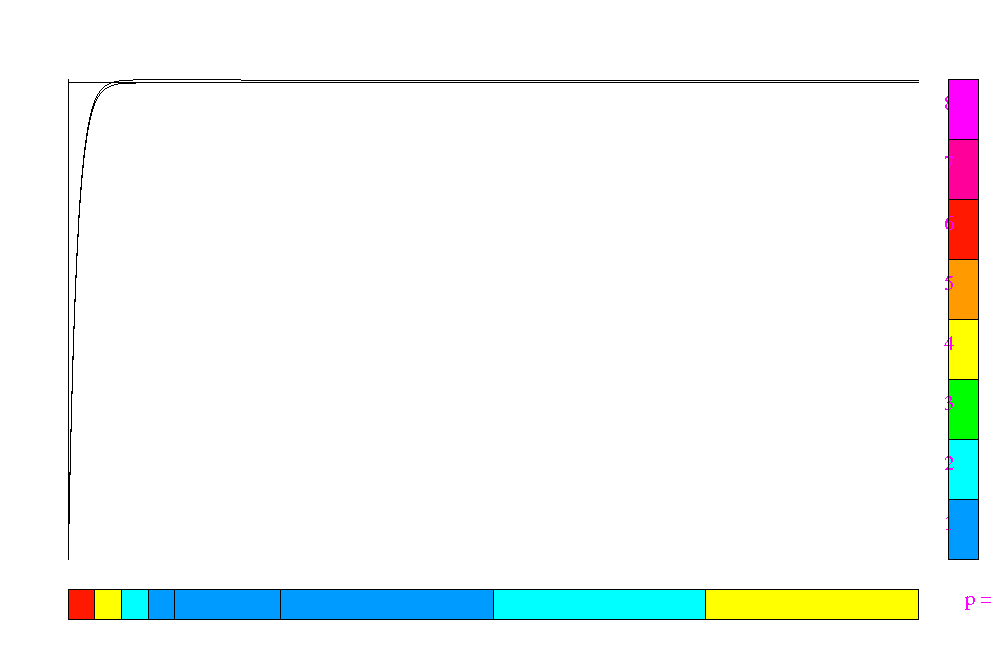
\includegraphics[scale=.175]{figs/opt.png}
\caption{$v$ and $\tau$ components of the 1D optimal test functions for flux $\widehat{f}_n$ on the \emph{right-hand} side of a unit element for $\epsilon = 0.01$. }
\label{fig:optTestBoundary}
\end{figure}
}

\frame{
\frametitle{Determining an alternative test norm}
Recall the convection-diffusion bilinear form
\begin{align*}
b\left(\left(u,\sigma, \widehat{u}, \widehat{f}_n\right),
\left( v, \tau \right)\right) = \left(u,\div \tau - \beta \cdot \grad
v\right)_{\Oh} + \left(\sigma, \epsilon^{-1} \tau + \grad v\right)_{\Oh}&\\
 - \LRa{\jump{\tau\cdot n}, \widehat{u} }_{\Gh} + \LRa{\widehat{f}_n,\jump{v} }_{\Gh}&,
\end{align*}
We recover $\nor{u}^2_{L^2(\Omega)}$ by choosing conforming $\LRp{v,\tau}$ satisfying the \emph{adjoint equations}
\begin{align*}
\div\tau - \beta \cdot \grad v   &= u\\
\frac{1}{\epsilon}\tau + \grad v &= 0
\end{align*}
with boundary conditions s.t.\ $\LRa{\jump{\tau\cdot n}, \widehat{u} }_{\Gamma}$ and $\LRa{ \widehat{f}_n,\jump{v} }_{\Gamma}$ vanish.
}

\frame{
\frametitle{A robust bound}
``Necessary'' conditions for robustness --- let $\boldsymbol U = \LRp{u,\sigma,\widehat{u},\widehat{f}_n}$. Then, by choosing specific $\LRp{v,\tau}$ satisfying the adjoint equations,
\[
\nor{u}^2_{L^2(\Omega)} = b\LRp{{\boldsymbol U},\LRp{v,\tau}} = \frac{b\LRp{{\boldsymbol U},\LRp{v,\tau}}}{\nor{\LRp{v,\tau}}_V} \nor{\LRp{v,\tau}}_V \leq \nor{\boldsymbol U}_E \nor{\LRp{v,\tau}}_V
\]
Let $\lesssim$ denote a robust bound - \textcolor{red}{if $ \nor{\LRp{v,\tau}}_V \lesssim \|u\|_{L^2(\Omega)}$}, then we have that
\[
\nor{u}_{L^2(\Omega)} \lesssim \nor{\boldsymbol U}_E
\]
\textbf{Main idea: the \textcolor{red}{test norm} should measure \textcolor{red}{adjoint solutions} robustly.}
}

\frame{
\frametitle{Choice of inflow boundary condition}

\begin{columns}
\begin{column}{.49\textwidth}
We impose the standard outflow wall boundary condition on $u$. For inflow boundary condition: 
\begin{itemize}
\item{} The standard choice of inflow boundary condition: $u = u_0$.
\item{} We impose the non-standard inflow condition: $\widehat{f}_n \coloneqq \beta_n u - \sigma_n \approx \beta_n u_0$ on $\Gamma_{\rm in}$.
\end{itemize}
\end{column}

\begin{column}{.49\textwidth}
\begin{figure}
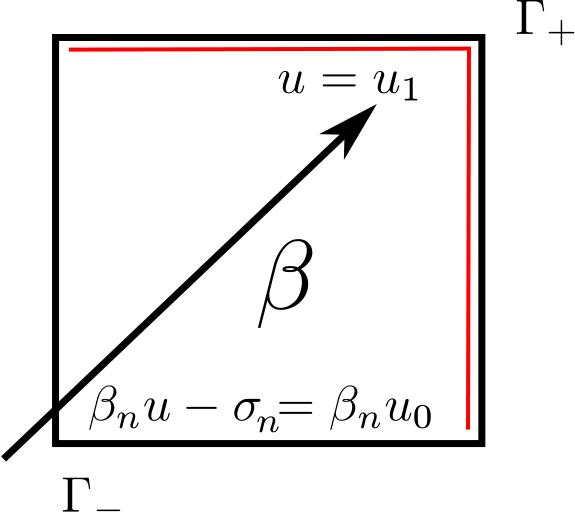
\includegraphics[scale=.23]{figs/primal.png}
\caption{Non-standard inflow.}
\end{figure}
\end{column}
\end{columns}
When $\sigma_n \approx 0$ near the inflow, condition on $\widehat{f}_n$ approximates condition on $u$. 

}

\frame{
\frametitle{Dirichlet inflow boundary condition}
Standard choice of boundary condition: $u = u_0$ on inflow boundary $\Gamma_{\rm in}$, induces boundary layers in adjoint problems, \textcolor{red}{$\nor{\beta\cdot \grad v}_{L^2} = O(\epsilon^{-1})$}.
\begin{figure}[h!]
\centering
\subfigure[Primal problem]{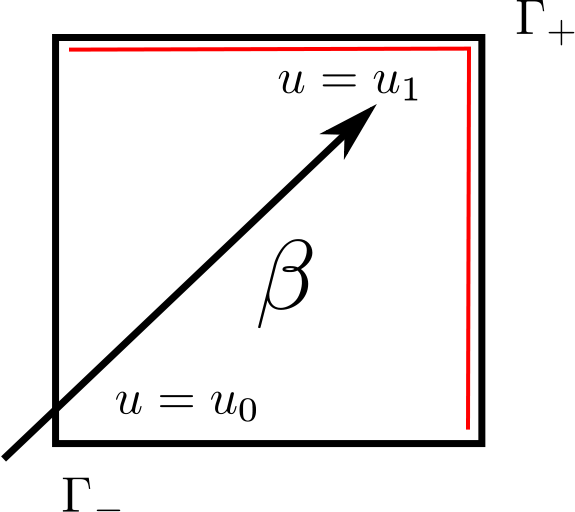
\includegraphics[scale=.23]{figs/primalDir.png}}
\subfigure[Adjoint problem]{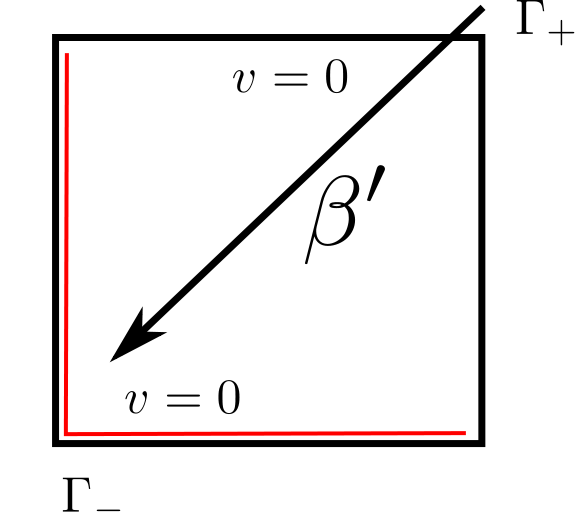
\includegraphics[scale=.23]{figs/adjointDir.png}}
\caption{For the standard Dirichlet inflow condition, the solution to the adjoint problem can develop strong boundary layers at the outflow of the adjoint problem. }
\end{figure}
}

\frame{
\frametitle{New inflow boundary condition on $\widehat{f}_n$}
Non-standard choice of boundary condition: $\widehat{f}_n = \beta_n u_0$ on $\Gamma_{\rm in}$, induces smoother adjoint problems, \textcolor{red}{$\nor{\beta\cdot \grad v}_{L^2} = O(1)$}.
\begin{figure}[h!]
\centering
\subfigure[Primal problem]{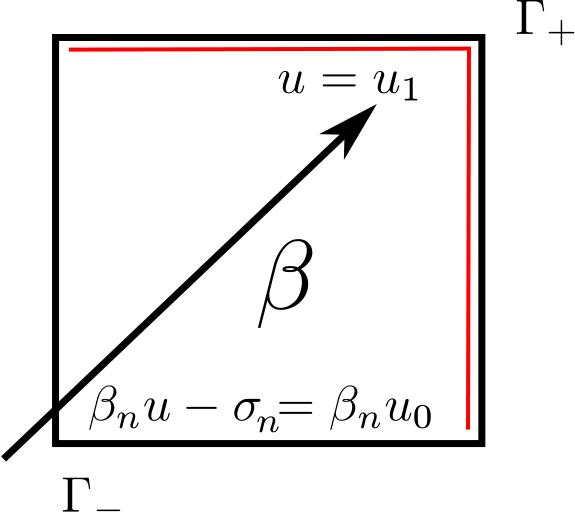
\includegraphics[scale=.23]{figs/primal.png}}
\subfigure[Adjoint problem]{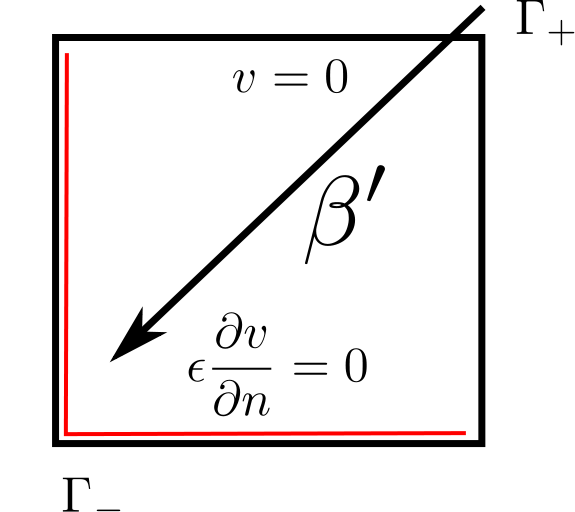
\includegraphics[scale=.23]{figs/adjoint.png}}
\caption{Under the new inflow condition, the wall-stop boundary condition is relaxed to a zero-stress condition at the outflow boundary of the adjoint problem.}
\end{figure}
}

\frame{
\frametitle{Test norms and adjoint solutions}
\textbf{Intuition:} the effectiveness of DPG under a test norm is governed by how a \textbf{specific test norm} measures the \textbf{solutions of the adjoint problem}. 

\begin{figure}[!h]
\centering
\subfigure[Dirichlet inflow]{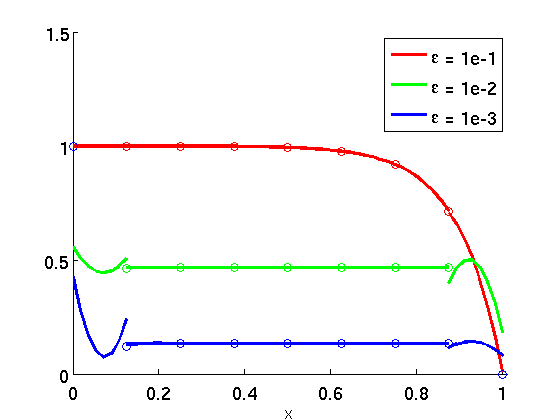
\includegraphics[scale=.35]{figs/dirichletBC.png}}
\subfigure[``Convection'' inflow]{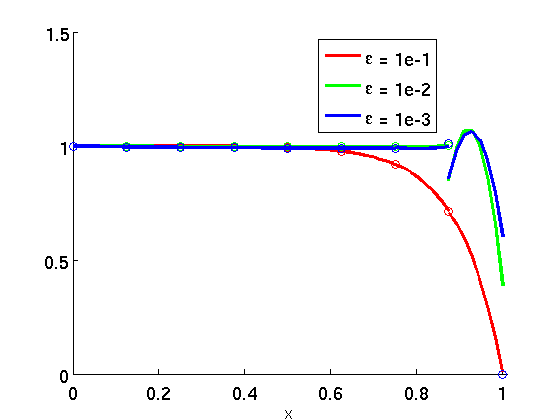
\includegraphics[scale=.35]{figs/newBC.png}}
\caption{DPG solutions to convection-diffusion for both inflow conditions using an $H^1$ test norm.}
\end{figure}
}

%\frame{
%\frametitle{``Building blocks'' norm}
%Test norm quantities are robustly bounded from above by $\nor{u}_{L^2(\Omega)}$.  
%\[
%\|\left(v,\tau\right)\|_{V,K}^2 = \|v\|^2 + \epsilon \|\grad v\|^2 + \|\beta \cdot \grad v\|^2 + \| \div \tau\|^2 + \frac{1}{\epsilon}\|\tau\|^2.
%\]
%Problem: boundary layers in optimal test functions:
%\begin{figure}[!h]
%\centering
%\subfigure{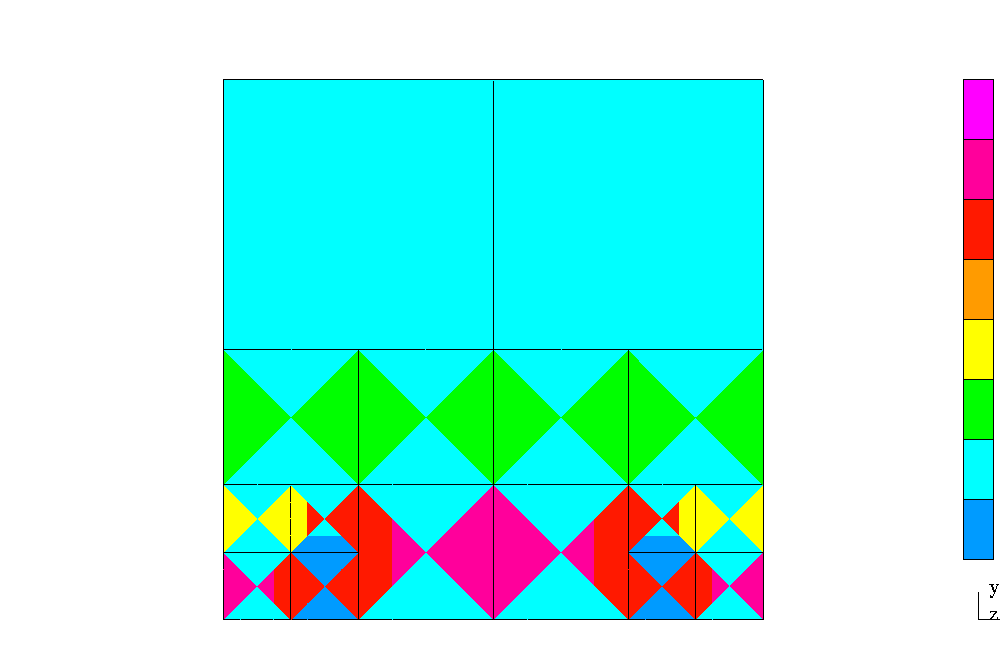
\includegraphics[scale=.15]{figs/mesh1.png}}
%\subfigure{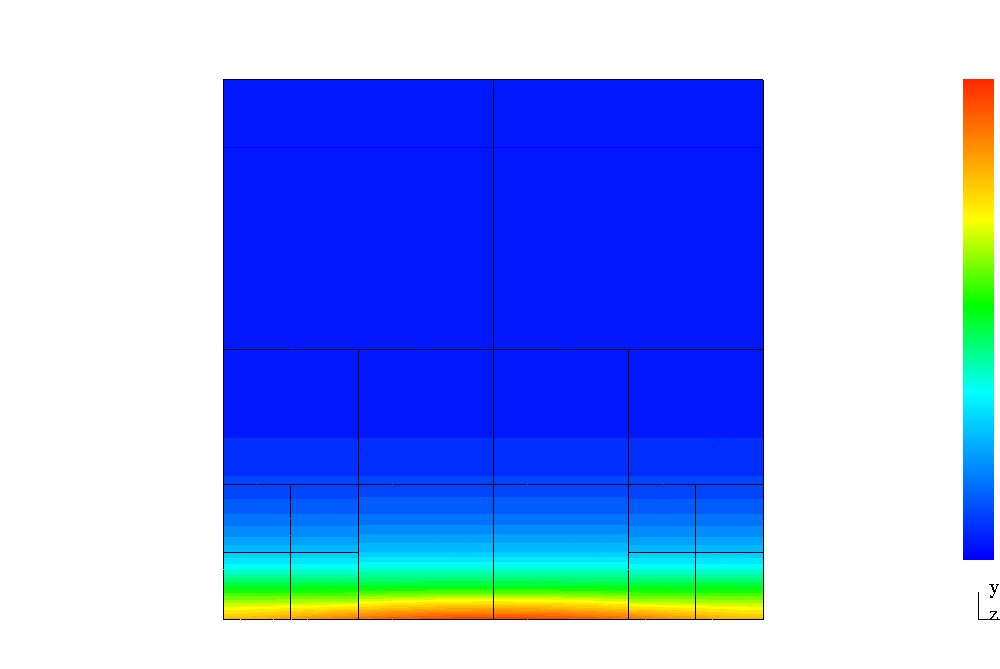
\includegraphics[scale=.15]{figs/sol1.png}}
%\caption{The $v$ component of the optimal test function corresponding to flux $\widehat{u} = x(1-x)$ on the bottom side of a unit element for $\epsilon = 0.01$.}
%\label{fig:boundaryTest}
%\end{figure}
%}
\frame{
\frametitle{Adjoint estimates, or ``norm building blocks''}
For solutions $(v,\tau)$ of the adjoint equations, the following quantities are robustly bounded from above by $\nor{u}_{L^2(\Omega)}$.  
\begin{align*}
&\|v\|, \sqrt{\epsilon} \|\grad v\|, \|\beta \cdot \grad v\| \\
&\| \div \tau\|, \frac{1}{\sqrt{\epsilon}}\|\tau\|.
\end{align*}
We will construct a test norm through a combination of the above quantities, such that
\begin{itemize}
\item $v$ and $\tau$ decoupled (no systems).
\item Coefficients are of equal order after transforming to the unit element (no boundary layers).
\end{itemize}
}
\frame{
\frametitle{Mesh-scaled test norms}
Our test norm, as defined over a single element $K$, is now
\begin{align*}
\|\left(v,\tau\right)\|_{V,K}^2 = \min\left\{\frac{\epsilon}{|K|},1\right\}\|v\|^2 + \epsilon \|\grad v\|^2 + \|\beta \cdot \grad v\|^2 +&\\
\| \div \tau\|^2 + \min\left\{\frac{1}{\epsilon},\frac{1}{|K|}\right\}\|\tau\|^2&.
\end{align*}
which induces the proven \emph{robust} bound\footnote{\bibentry{DPGrobustness2}}
\[
\nor{u}_{L^2(\Omega)}+ \nor{\sigma}_{L^2(\Omega)} + \epsilon\nor{\widehat{u}} + \sqrt{\epsilon} \nor{\widehat{f}_n} \lesssim \nor{\LRp{u,\sigma,\widehat{u},\widehat{f}_n}}_E.
\]
}

\frame{
\frametitle{Erikkson-Johnson model problem}

On domain $\Omega = [0,1]^2$, with $\beta = (1,0)^T$, $ f = 0$ and boundary conditions
\begin{align*}
\widehat{\beta_nu - \sigma_n} &= \widehat{f}_n = u_0, \quad \beta_n \leq 0\\
\widehat{u} &= 0, \quad \beta_n > 0
\end{align*}

%Separation of variables gives an analytic solution. 
All numerical experiments done using Camellia codebase.\footnote{\bibentry{Camellia}}
%\[
%u(x,y) = C_0 + \sum_{n=1}^\infty C_n \frac{\exp(r_2(x-1)-\exp(r_1(x-1)))}{r_1\exp(-r2) - r_2\exp(-r1)}\cos(n\pi y)
%\]
\begin{figure}
\centering
\subfigure{
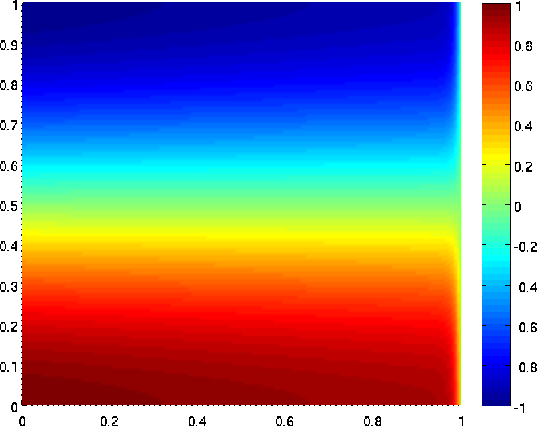
\includegraphics[scale=.23]{figs/wallBC_exact_u.png}
}
\subfigure{
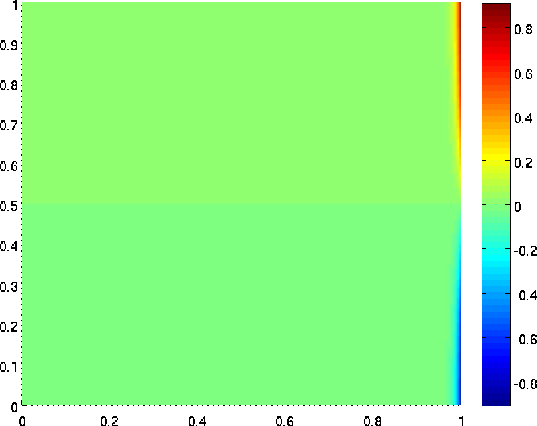
\includegraphics[scale=.23]{figs/wallBC_exact_sigx.png}
}
\subfigure{
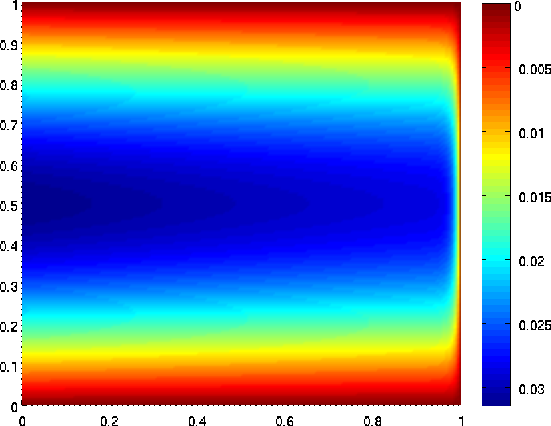
\includegraphics[scale=.23]{figs/wallBC_exact_sigy.png}
}
\caption{Exact solution for $u$, $\sigma_x$, and $\sigma_y$ for $\epsilon = .01$, $C_1 = 1$, $C_n=0$, $n\neq 1$}
\end{figure}
}

\frame{
\frametitle{Error rates}
\begin{figure}
\centering
\subfigure{
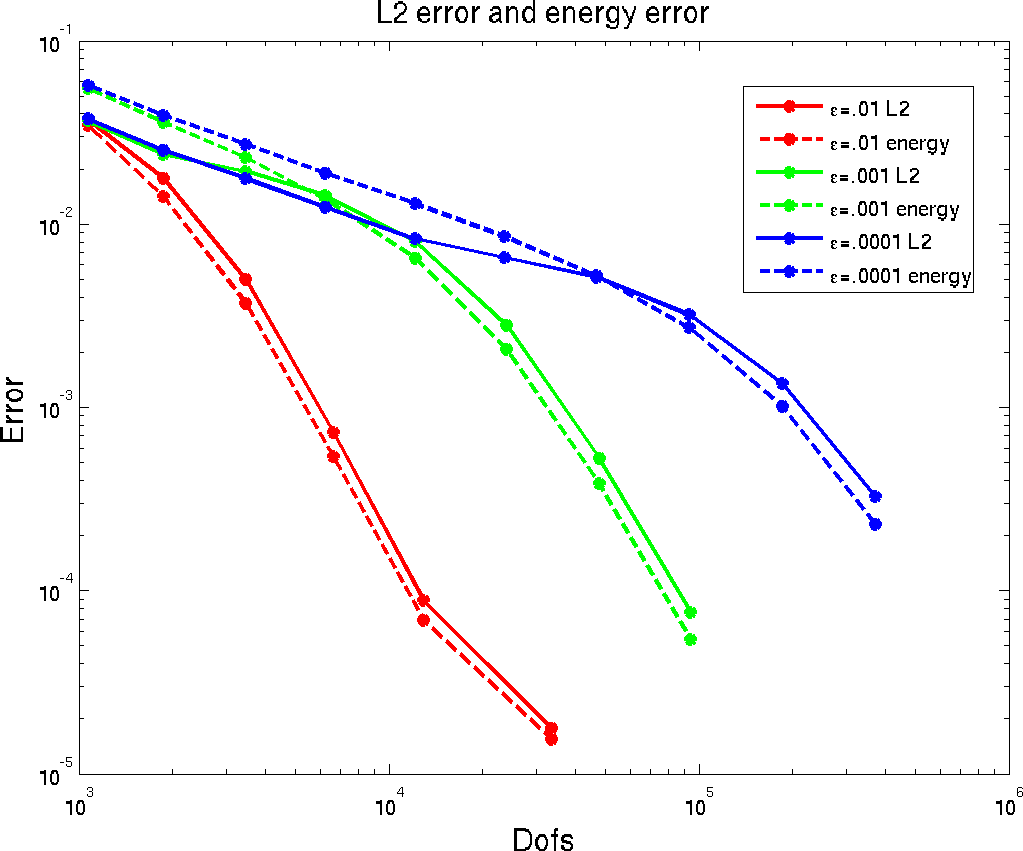
\includegraphics[scale=.33]{figs/errorrates_wallBC.png}
}
\subfigure{
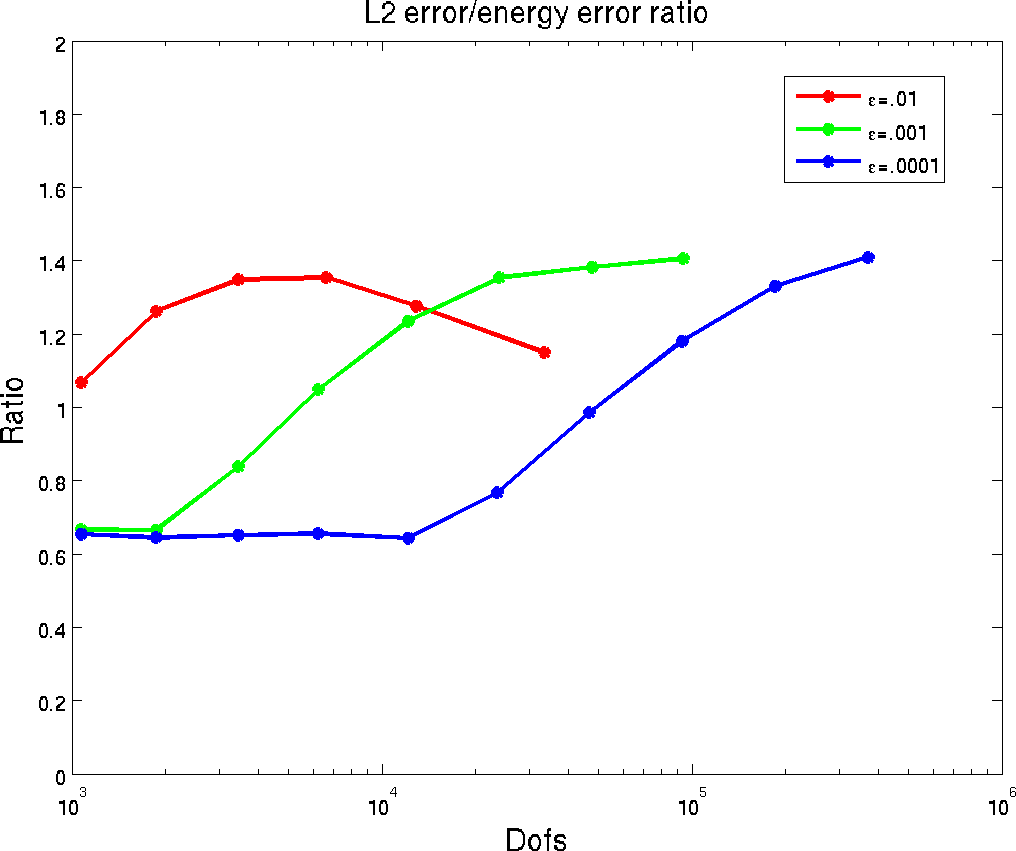
\includegraphics[scale=.33]{figs/L2energyratio_wallBC.png}
}
%\subfigure{
%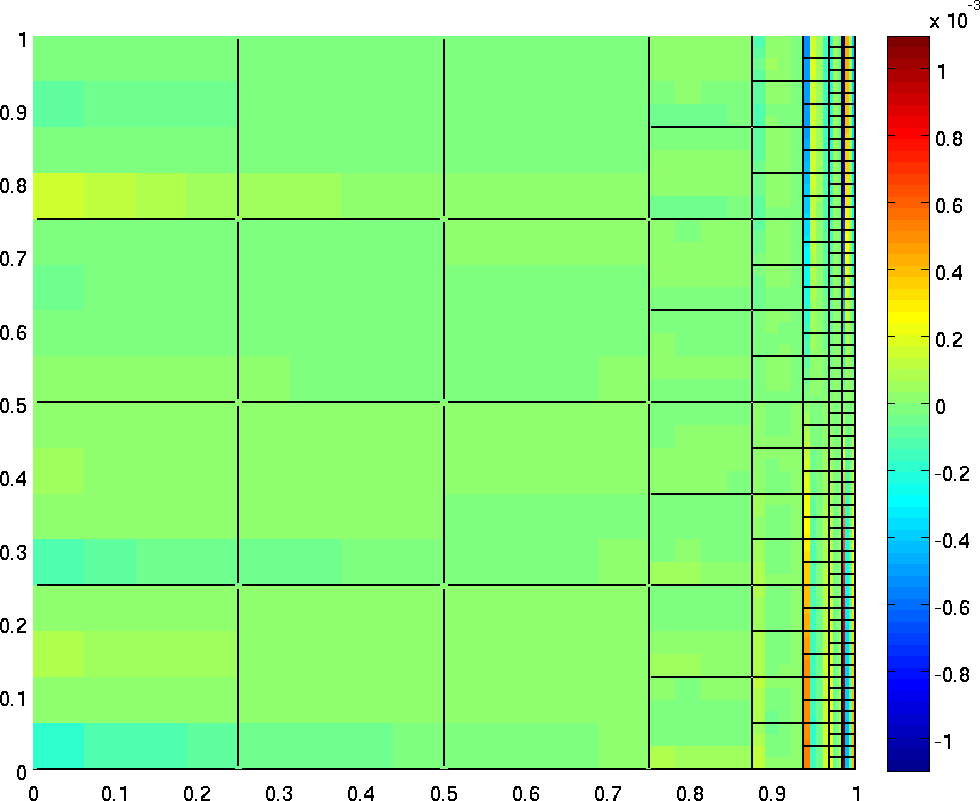
\includegraphics[scale=.22]{figs/u_pointdiff_wallBC.png}
%}
\caption{$L^2$/energy errors and their ratio for $\epsilon = .01, .001, .0001$.}
\end{figure}
}

%\frame{
%\frametitle{Regularization}
%Discontinuous inflow conditions on $\widehat{f_n}$, out of alignment with mesh. Boundary condition $\epsilon \grad u \cdot n = 0$ at outflow.
%\begin{figure}
%\centering
%\subfigure{
%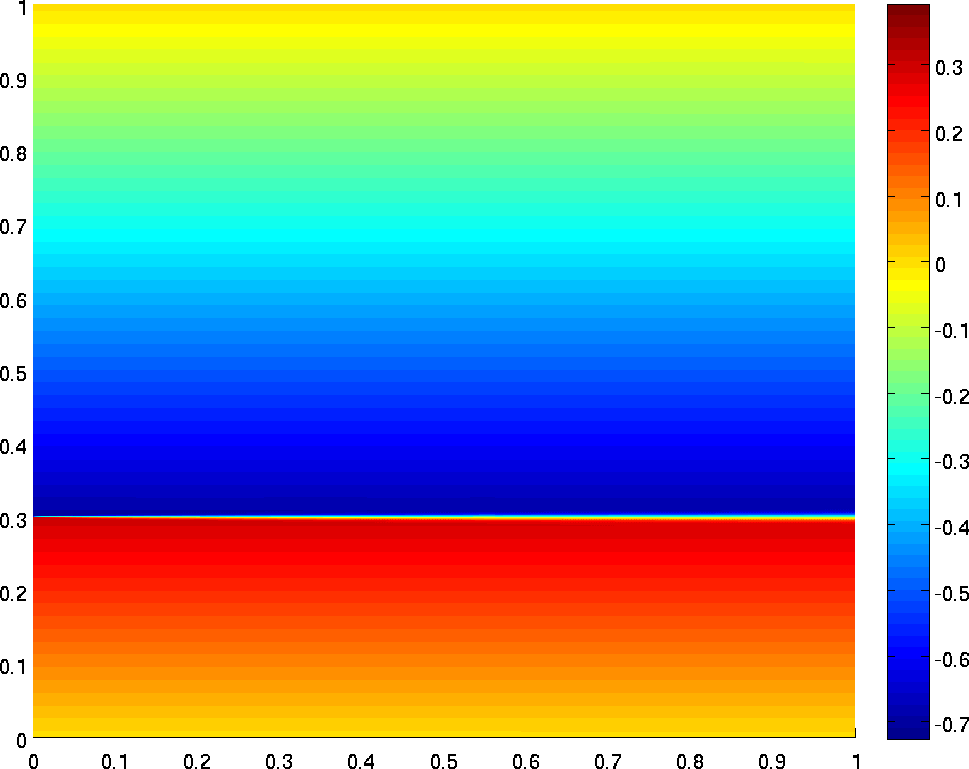
\includegraphics[scale=.33]{figs/discontinuous.png}
%}
%\subfigure{
%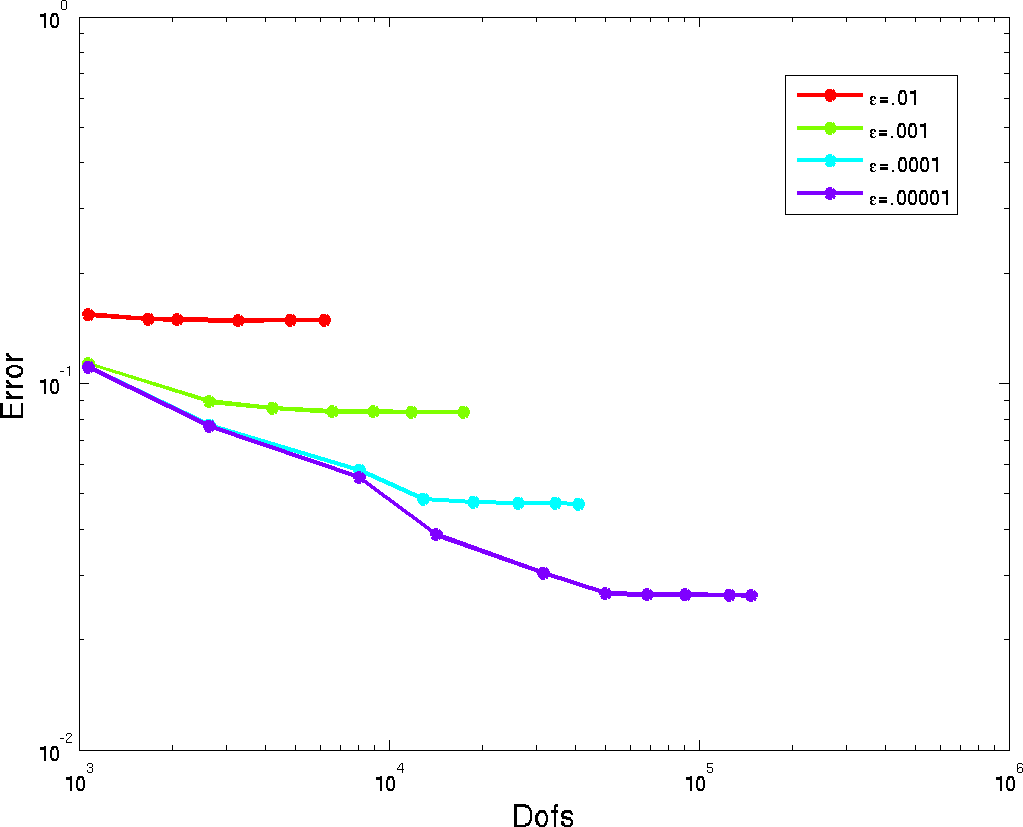
\includegraphics[scale=.305]{figs/discontinuousL2rates.png}
%}
%\caption{Discontinuous hat inflow data with $\epsilon = 1e-5$, convection solution errors.}
%\end{figure}
%}
\frame{
\frametitle{Local conservation}
Given stiffness matrix $K$, can introduce Lagrange multipliers to enforce element-wise constraints, leading to the saddle point problem
\[
\arr{K}{B}{B^T}{0}\vecttwo{u}{\lambda} = \vecttwo{f}{c}.
\]
where the Lagrange multipliers $\lambda$ can be locally condensed. We use the test norm
\begin{align*}
\|\left(v,\tau\right)\|_{V,K}^2 = \left|\int_K v\right|^2 + \epsilon \|\grad v\|^2 + \|\beta \cdot \grad v\|^2 +&\\
\| \div \tau\|^2 + \min\left\{\frac{1}{\epsilon},\frac{1}{|K|}\right\}\|\tau\|^2&.
\end{align*}
}

\frame{
\frametitle{Additional examples}
\begin{figure}
\centering
\subfigure[Advection skew]{
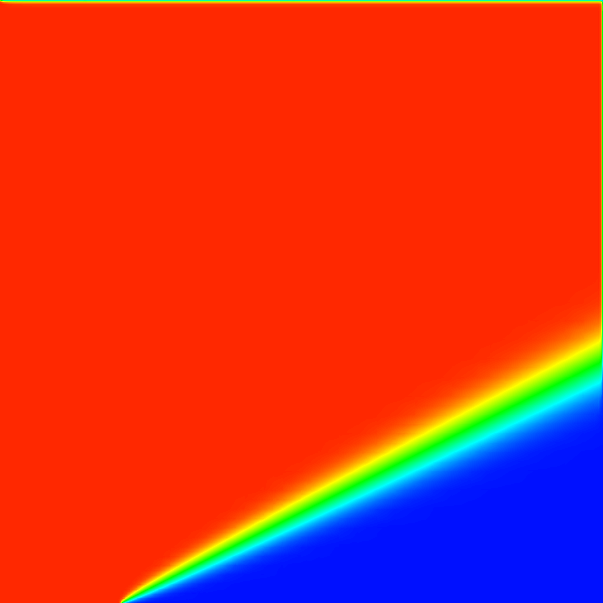
\includegraphics[scale = .175]{figs/Conservative/hughes.png}
}
\subfigure[Flow over a step]{
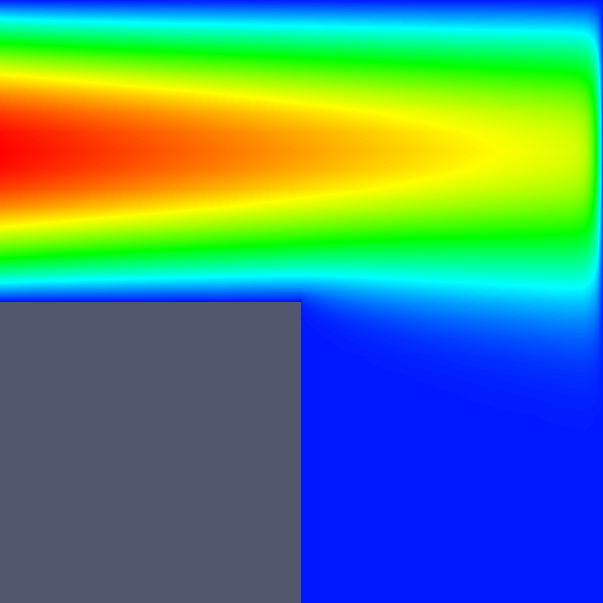
\includegraphics[scale = .175]{figs/Conservative/step.png}
}
\subfigure[Double glazing]{
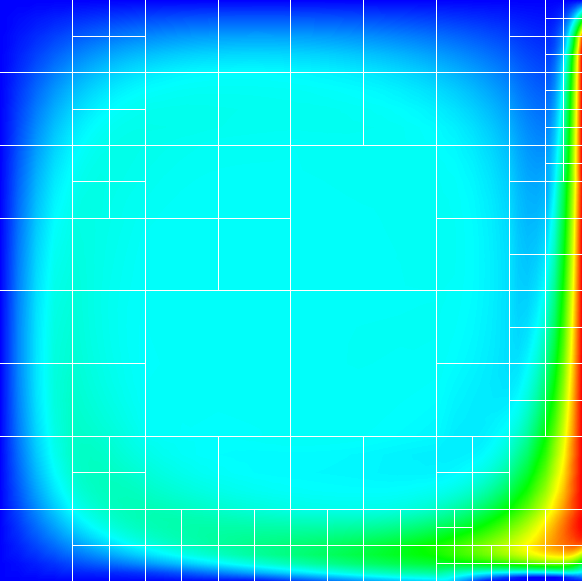
\includegraphics[scale = .182]{figs/Conservative/doubleGlazing.png}
}
\end{figure}
Locally conservative version of DPG performs very similarly to the standard DPG in all cases over a range of $\epsilon$. 
}

\frame{
\frametitle{Regularization}
For $\beta = (-y,x)^T$ on $\Omega = [-1,1]^2$. Ill posed in the convection setting. Similar tests have been done with discontinuous data.

\begin{figure}
\centering
\subfigure{

\includegraphics[scale=.21]{figs/vortex.png}
}
\subfigure{
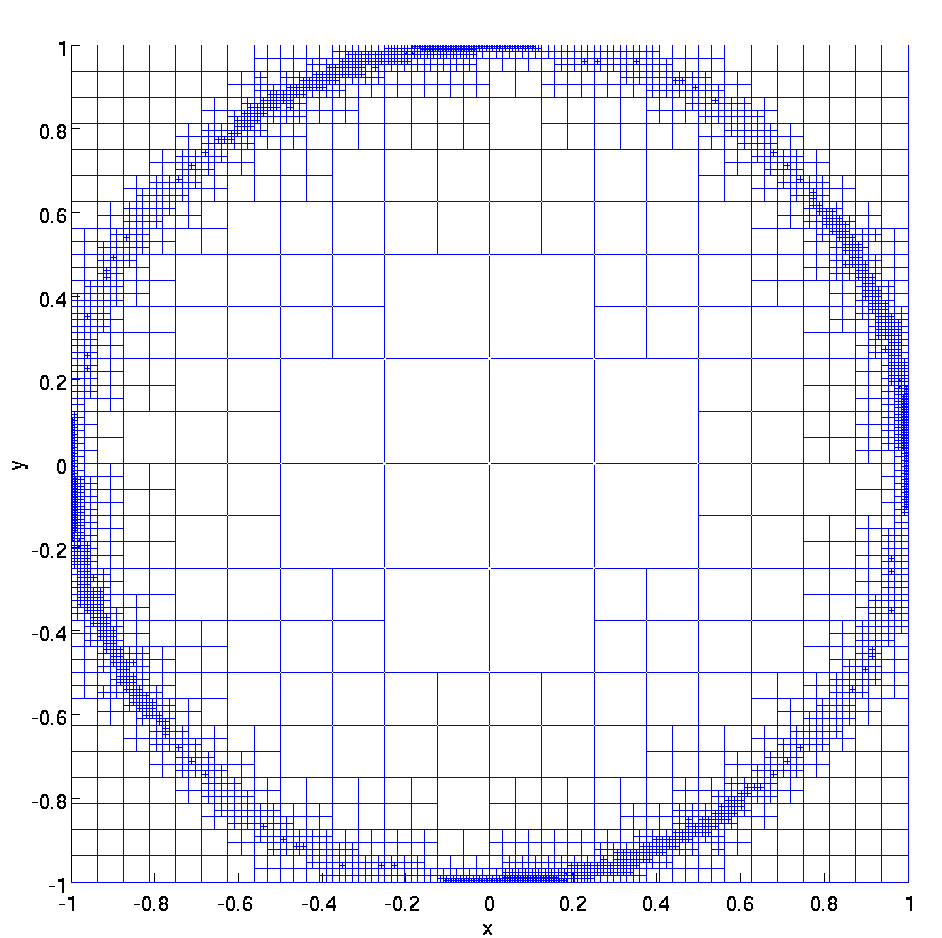
\includegraphics[scale=.2015]{figs/vortexMesh.png}
}
\caption{Steady vortex problem with $\epsilon = 1e-4$.}
\end{figure}
\vspace{-.25cm}
}

\frame{
\frametitle{Current work - Hemker problem}

\begin{figure}
\centering
\subfigure{
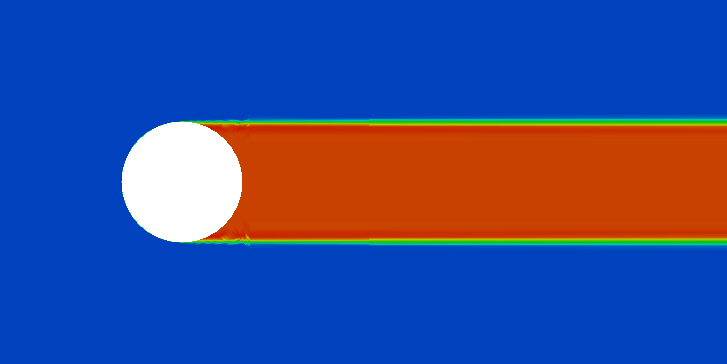
\includegraphics[scale = .225]{figs/Conservative/Hemker/WithoutMesh.png}
}
\subfigure{
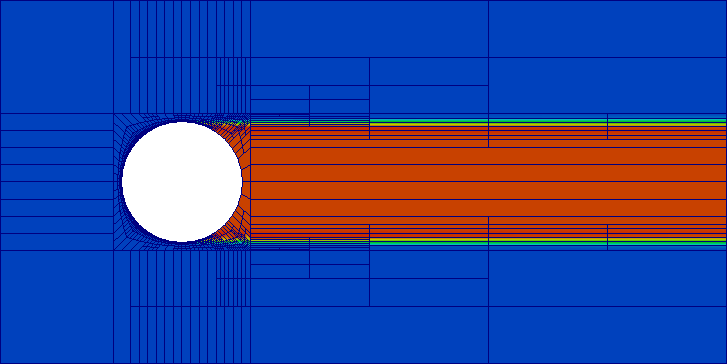
\includegraphics[scale = .225]{figs/Conservative/Hemker/WithMesh.png}
}
\caption{Convection-diffusion solution to flow over a cylinder at $\epsilon = 1e-4$.}
\end{figure}
}
\frame{
\frametitle{Current work - high-lift airfoil}
\begin{figure}
\centering
\subfigure{
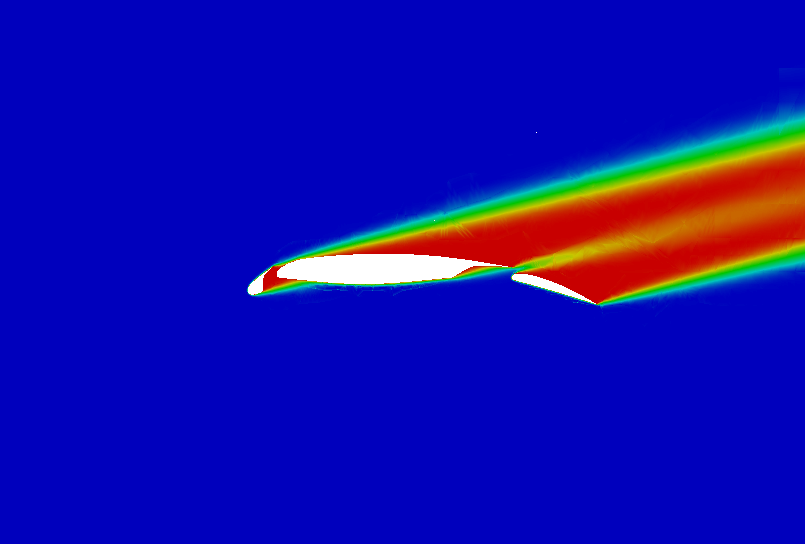
\includegraphics[scale = .1875]{figs/Conservative/Airfoil-Conservative-1E-3/solution.png}
}
\subfigure{
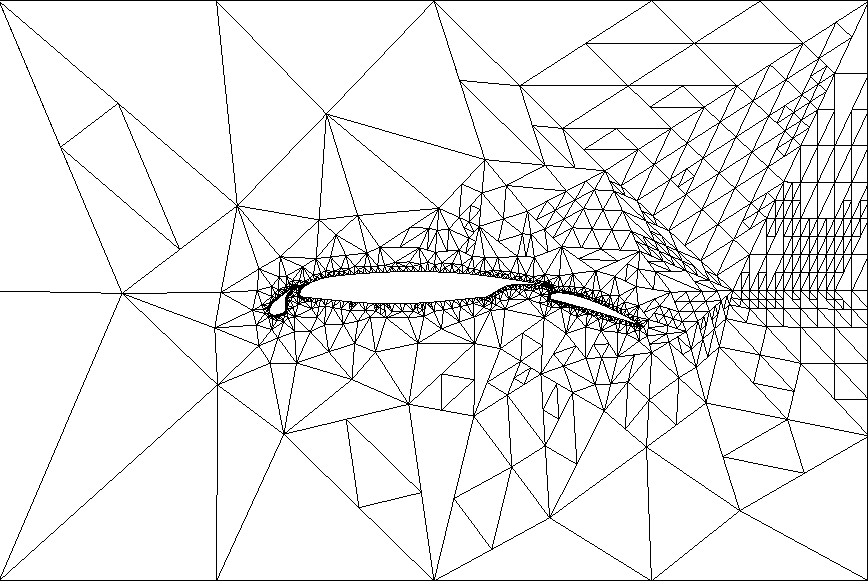
\includegraphics[scale = .175]{figs/Conservative/Airfoil-Conservative-1E-3/mesh7.png}
}
\caption{Convection-diffusion solution over the high-lift airfoil, with advection at an angle, $\epsilon = 1e-3$, with $p=3$. Mesh is generated by \emph{Triangle}.}
\end{figure}
}

\section{DPG for nonlinear problems}
\frame{
\frametitle{DPG for nonlinear problems}

Given some linearization technique (typically Newton-Raphson and pseudo-timestepping linearization), we measure 
\begin{itemize}
\item size of the linearized update $\Delta u$
\[
\|\Delta u\|_E \coloneqq \nor{B_u\Delta u}_{V'} = \nor{R_V^{-1} B_u\Delta u}_V 
\]
\item the nonlinear residual 
\[
\nor{R(u)}_E \coloneqq \nor{B(u) - \ell}_{V'}  = \nor{R_V^{-1}\LRp{B(u)-\ell}}_V 
\]
\end{itemize}
Preliminary experiments were done in 1D\footnote{\bibentry{DPGNS_1d}} and space-time.\footnote{\bibentry{DPGspacetime}}
}

\frame{
\frametitle{2D test case: Burgers equation}
\begin{columns}
\begin{column}{.48\textwidth}
\vspace{-.5cm}
\[
\pd{\left(u^2/2\right)}{x} + \pd{u}{y} + \epsilon \Delta u = f
\]
Burgers equation can be written with $\beta(u) = \LRp{u/2,1}$
\begin{align*}
\div\left(\beta(u)u-\sigma\right) &=f \\
\frac{1}{\epsilon}\sigma - \grad u &=0.
\end{align*}
i.e.\ nonlinear convection-diffusion on domain $[0,1]^2$.
\end{column}
\begin{column}{.48\textwidth}
\begin{figure}[!h]
\centering
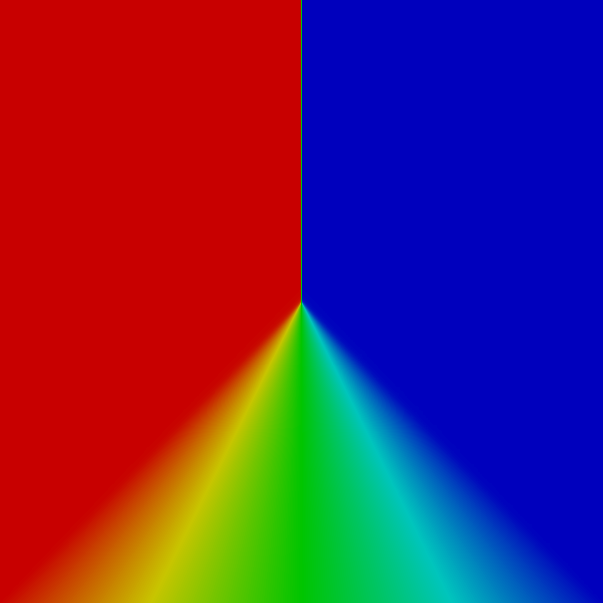
\includegraphics[scale = .22]{figs/burgers.png}
\caption{Shock solution for Burgers' equation, $\epsilon = 1e-4$, using Newton-Raphson.}
\end{figure}
\end{column}
\end{columns}
}
\frame{
Adaptivity begins with a cubic $4\times 4$ mesh.
\begin{figure}[!h]
\centering
\subfigure{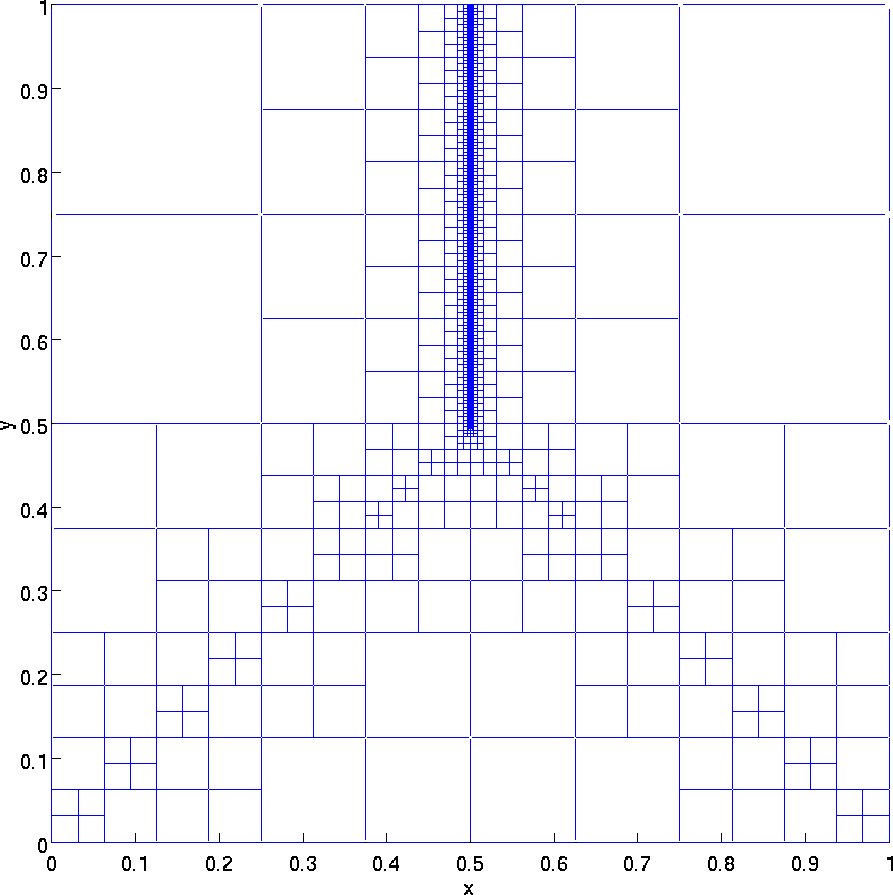
\includegraphics[scale=.2]{figs/burgersMesh.png}}
\subfigure{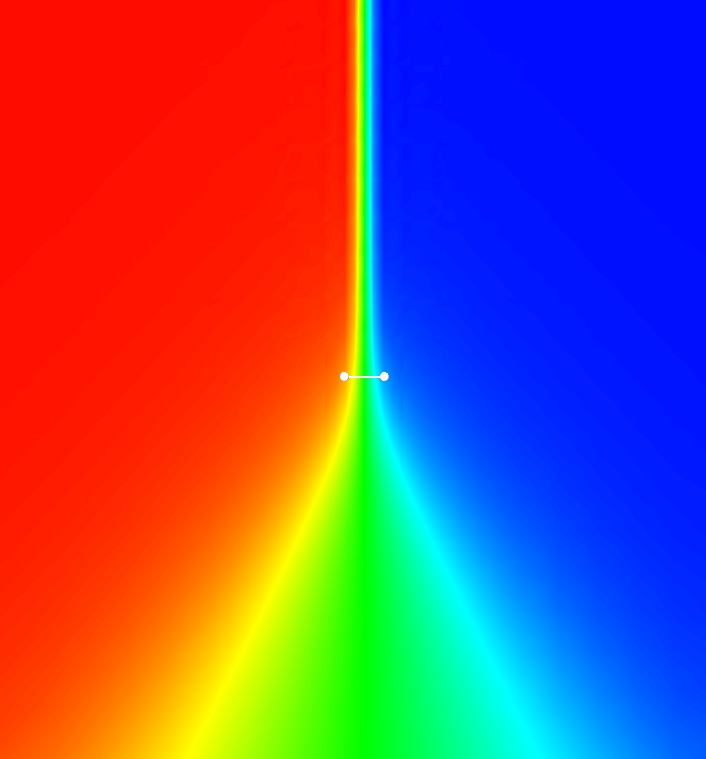
\includegraphics[scale=.2]{figs/burgersZoom.png}}
\caption{Adaptive mesh after 9 refinements, and zoom view at point (.5,.5) with shock formation and $1e-3$ width line for reference.}
\end{figure}
}

\frame{
\frametitle{2D Compressible Navier-Stokes equations (ideal gas)}
Given density $\rho$, velocities $\mathbf{u} = \LRp{u_1,u_2}$ and temperature $T$,
\begin{align*}
\div \vecttwo{\rho u_1 }{\rho u_2} &= 0\\
\div \left(\vecttwo{\rho u_1^2+p }{\rho u_1 u_2} - \boldsymbol \sigma_{1}\right) &=0\\
\div \left(\vecttwo{\rho u_1 u_2}{\rho u_2^2+p } - \boldsymbol \sigma_{2}\right) &=0\\
\div \left(\vecttwo{((\rho e)+p)u_1}{((\rho e)+p)u_2} - \boldsymbol\sigma \mathbf{u} + \vec{q}\right) &=0\\
\frac{1}{2\mu} \boldsymbol \sigma - \frac{\lambda}{4\mu (\mu + \lambda)} { \rm tr}(\boldsymbol \sigma) \boldsymbol I &= \grad \mathbf{u} - \Reyn \, \boldsymbol w\\
\frac{1}{\kappa}\vec{q} &= \grad T
\end{align*}
}

\frame{
\frametitle{Stress law}
$\boldsymbol\sigma$ for a Newtonian fluid: $\sigma_{ij} = \mu(u_{i,j} + u_{j,i}) + \lambda u_{k,k} \delta_{ij}$.
%We can invert the stress tensor under isotropic and plane strain assumptions to get
\[
\frac{1}{2}\left(\grad  U + \grad ^T  U\right) = \frac{1}{2\mu} \sigma_{ij} - \frac{\lambda}{4\mu (\mu + \lambda)} \sigma_{kk}\delta_{ij}
\]
The symmetric part of the gradient is
\[
\frac{1}{2}\left(\grad  U + \grad ^T  U\right) = \grad  U - \boldsymbol w
\]
Our final form is
\begin{align*}
\grad  U - \boldsymbol w= \frac{1}{2\mu} \boldsymbol \sigma - \frac{\lambda}{4\mu (\mu + \lambda)} { \rm tr}(\boldsymbol \sigma) \boldsymbol I.
\end{align*}
By enforcing strong symmetry of $\boldsymbol \sigma$, taking the antisymmetric part implicitly defines $\boldsymbol w$ to be the antisymmetric part of $\grad u$. 
}

\frame{
\frametitle{Extrapolation of test norms}
%\begin{columns}
%\begin{column}{.48\textwidth}
Convection-diffusion:
\begin{align*}
\div \left(\beta u - \sigma\right) &= f\\
\frac{1}{\epsilon}\sigma - \grad u &= 0.
\end{align*}
Navier-Stokes: defining vector variables $U = \{\rho,u_1,u_2,T\}$ and $\Sigma = \{{\boldsymbol \sigma},\mathbf{q},w\}$,
\begin{align*}
\div \left(A_{\rm invisc}U - A_{\rm visc}\Sigma\right) &= R_{\rm conserv}(U,\Sigma)\\
E_{\rm visc} \Sigma - \grad U &= R_{\rm constit}(U,\Sigma)
\end{align*}
where $R_{\rm conserv}(U,\Sigma)$ and $R_{\rm constit}(U,\Sigma)$ are the conservation/constitutive residuals.
}

\frame{
\frametitle{Test norms over one element}
Convection-diffusion:
\begin{align*}
\|\left(v,\tau\right)\|_{V,K}^2 =& \min\left\{\frac{\epsilon}{|K|},1\right\}\|v\|^2 + \|\beta \cdot \grad v\|^2 + \epsilon \|\grad v\|^2  \\
&+\| \div \tau\|^2 + \min\left\{\frac{1}{\epsilon},\frac{1}{|K|}\right\}\|\tau\|^2.
\end{align*}

Navier-Stokes: let $V$ and $W$ be vectors of test functions $v_i$ and $\tau_i$.
\begin{align*}
\|\left(V,W\right)\|_{V,K}^2 =& \min\left\{\frac{1}{\Reyn|K|},1\right\}\nor{V}^2  + \nor{A_{\rm invisc}^T \grad V}^2 + \frac{1}{\Reyn} \nor{A_{\rm visc}^T\grad V}^2 \\
& + \nor{\div W}^2 + \min\left\{1,\frac{1}{\Reyn|K|}\right\}\nor{E_{\rm visc}^TW}^2.
\end{align*}
}

\frame{
\frametitle{Carter's flat plate problem}
\begin{columns}
\begin{column}{.49\textwidth}
\begin{figure}[!h]
\centering
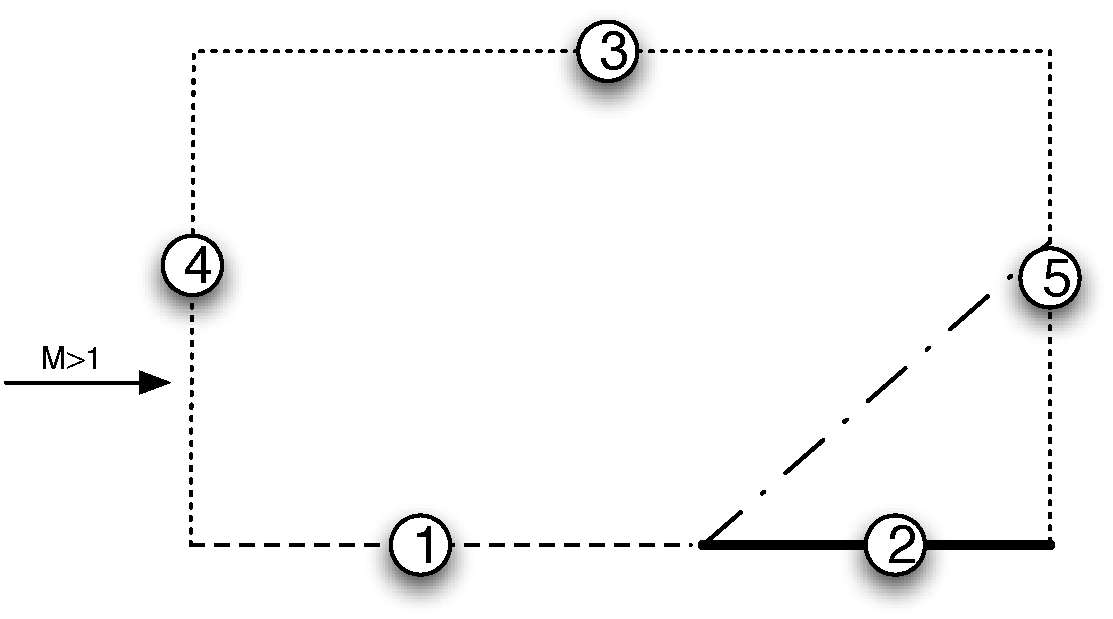
\includegraphics[scale=.32]{figs/flat_plate_BCs.pdf}
\caption{Carter flat plate problem on domain $[0,2]\times[0,1]$. Plate begins at $x=1$, ${\rm Re} = 1000$.}
\end{figure}
\end{column}
\begin{column}{.49\textwidth}
\begin{enumerate}
\item{} Symmetry boundary conditions.
\item{} Prescribed temperature and wall stagnation conditions.
\item{} Symmetry boundary conditions.
\item{} Inflow: conserved quantities specified using far-field values.
\item{} No outflow condition set.
\end{enumerate}
Stress/heat flux boundary conditions are set in terms of the momentum and energy fluxes. 
\end{column}
\end{columns}
}

\frame{
\frametitle{Refinement level 0}
\begin{figure}
\centering
\subfigure[$u_1$]{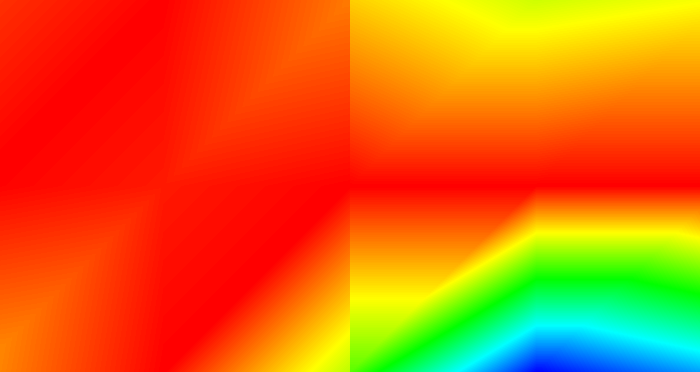
\includegraphics[scale = .23]{figs/propMovie/u0.png}}
\subfigure[$T$]{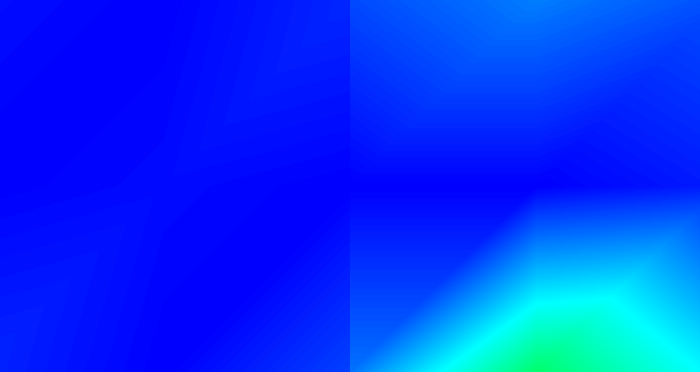
\includegraphics[scale = .23]{figs/propMovie/T0.png}}
\subfigure{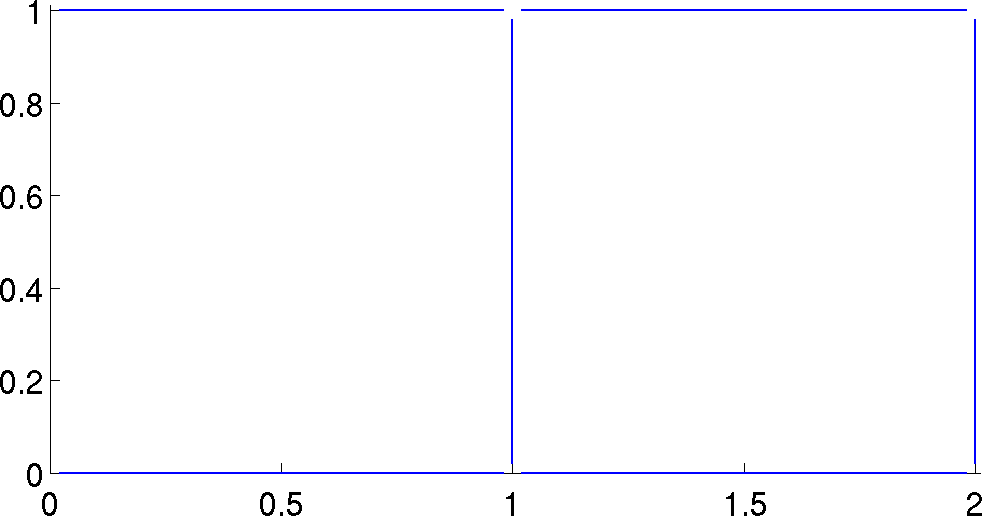
\includegraphics[scale = .35]{figs/propMovie/Mesh0.png}}
\end{figure}
}
\setcounter{subfigure}{0}


\frame{
\frametitle{Refinement level 1}
\begin{figure}
\centering
\subfigure[$u_1$]{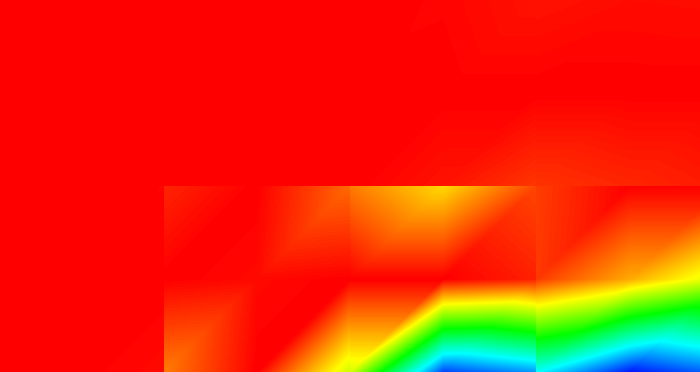
\includegraphics[scale = .23]{figs/propMovie/u1.png}}
\subfigure[$T$]{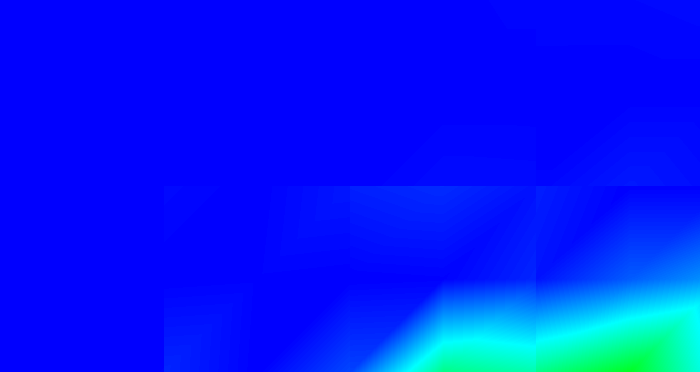
\includegraphics[scale = .23]{figs/propMovie/T1.png}}
\subfigure{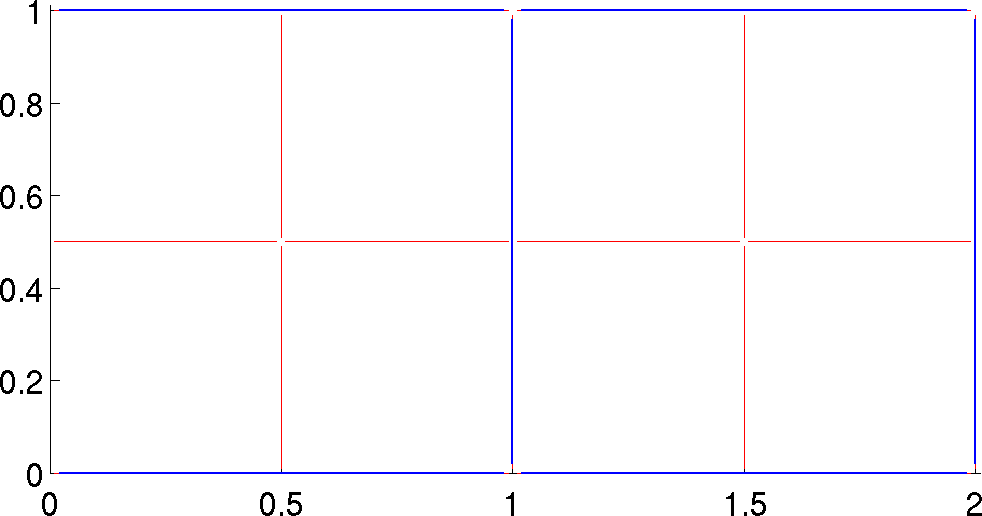
\includegraphics[scale = .35]{figs/propMovie/Mesh1.png}}
\end{figure}
}
\setcounter{subfigure}{0}


\frame{
\frametitle{Refinement level 2}
\begin{figure}
\centering
\subfigure[$u_1$]{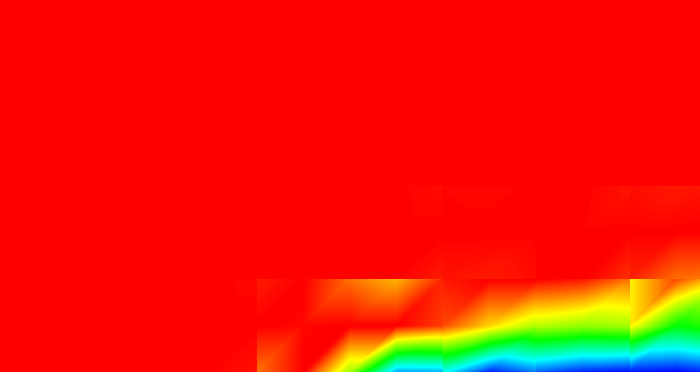
\includegraphics[scale = .23]{figs/propMovie/u2.png}}
\subfigure[$T$]{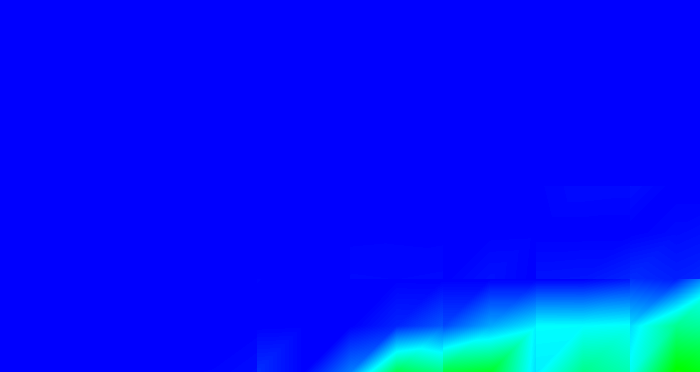
\includegraphics[scale = .23]{figs/propMovie/T2.png}}
\subfigure{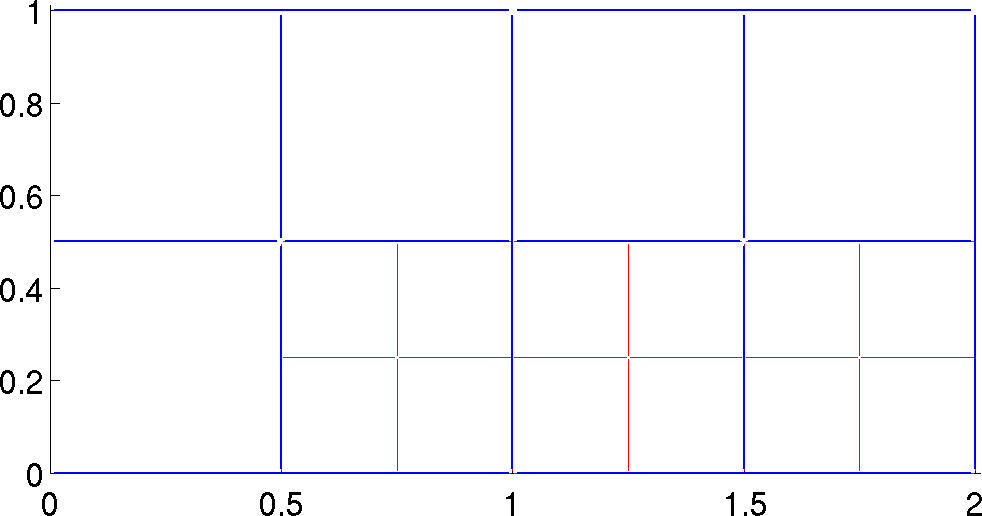
\includegraphics[scale = .35]{figs/propMovie/Mesh2.png}}
\end{figure}
}
\setcounter{subfigure}{0}


\frame{
\frametitle{Refinement level 3}
\begin{figure}
\centering
\subfigure[$u_1$]{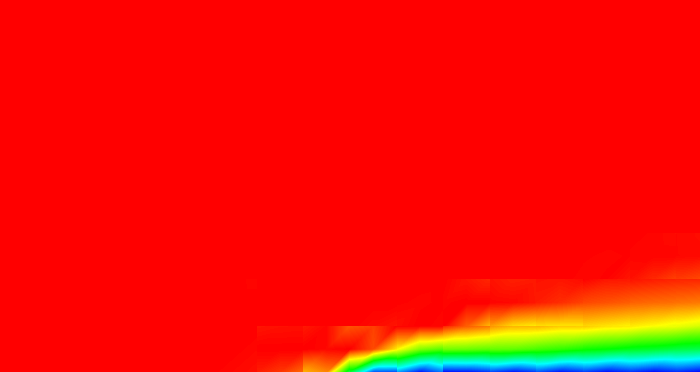
\includegraphics[scale = .23]{figs/propMovie/u3.png}}
\subfigure[$T$]{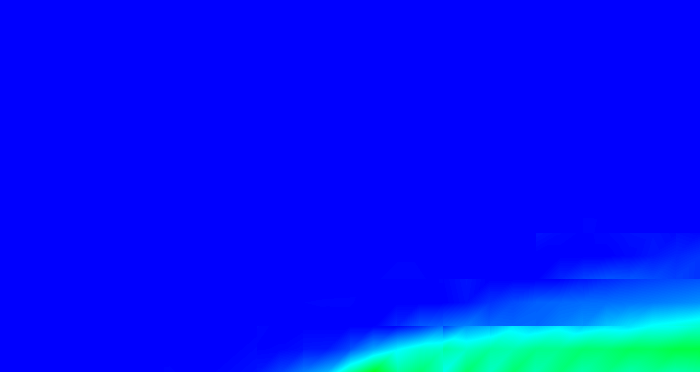
\includegraphics[scale = .23]{figs/propMovie/T3.png}}
\subfigure{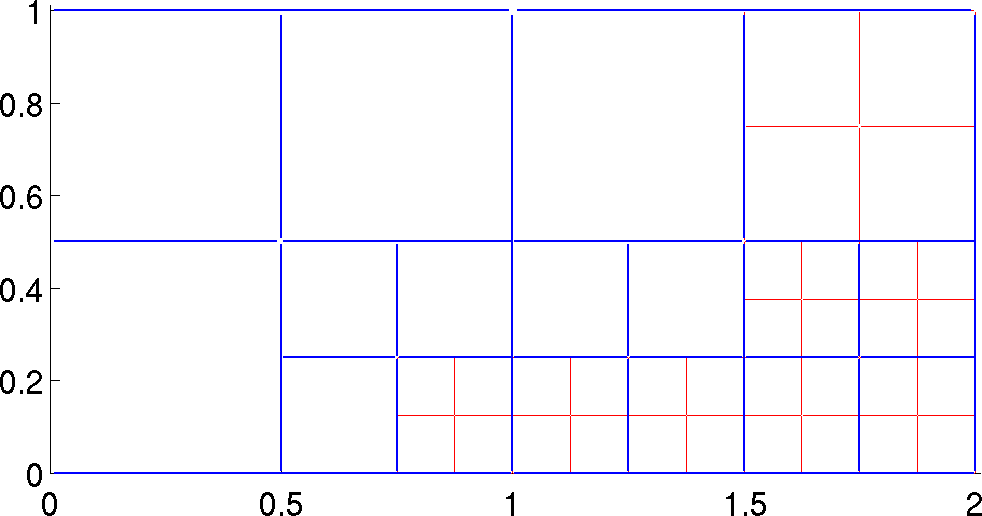
\includegraphics[scale = .35]{figs/propMovie/Mesh3.png}}
\end{figure}
}
\setcounter{subfigure}{0}



\frame{
\frametitle{Refinement level 4}
\begin{figure}
\centering
\subfigure[$u_1$]{\includegraphics[scale = .23]{figs/propMovie/u4.png}}
\subfigure[$T$]{\includegraphics[scale = .23]{figs/propMovie/T4.png}}
\subfigure{\includegraphics[scale = .35]{figs/propMovie/Mesh4.png}}
\end{figure}
}
\setcounter{subfigure}{0}



\frame{
\frametitle{Refinement level 5}
\begin{figure}
\centering
\subfigure[$u_1$]{\includegraphics[scale = .23]{figs/propMovie/u5.png}}
\subfigure[$T$]{\includegraphics[scale = .23]{figs/propMovie/T5.png}}
\subfigure{\includegraphics[scale = .35]{figs/propMovie/Mesh5.png}}
\end{figure}
}
\setcounter{subfigure}{0}

\frame{
\frametitle{Refinement level 6}
\begin{figure}
\centering
\subfigure[$u_1$]{\includegraphics[scale = .23]{figs/propMovie/u6.png}}
\subfigure[$T$]{\includegraphics[scale = .23]{figs/propMovie/T6.png}}
\subfigure{\includegraphics[scale = .35]{figs/propMovie/Mesh6.png}}
\end{figure}
}
\setcounter{subfigure}{0}



\frame{
\frametitle{Refinement level 7}
\begin{figure}
\centering
\subfigure[$u_1$]{\includegraphics[scale = .23]{figs/propMovie/u7.png}}
\subfigure[$T$]{\includegraphics[scale = .23]{figs/propMovie/T7.png}}
\subfigure{\includegraphics[scale = .35]{figs/propMovie/Mesh7.png}}
\end{figure}
}
\setcounter{subfigure}{0}


\frame{
\frametitle{Refinement level 8}
\begin{figure}
\centering
\subfigure[$u_1$]{\includegraphics[scale = .23]{figs/propMovie/u8.png}}
\subfigure[$T$]{\includegraphics[scale = .23]{figs/propMovie/T8.png}}
\subfigure{\includegraphics[scale = .35]{figs/propMovie/Mesh8.png}}
\end{figure}
}
\setcounter{subfigure}{0}

\frame{
\frametitle{Refinement level 9}
\begin{figure}
\centering
\subfigure[$u_1$]{\includegraphics[scale = .23]{figs/propMovie/u9.png}}
\subfigure[$T$]{\includegraphics[scale = .23]{figs/propMovie/T9.png}}
\subfigure{\includegraphics[scale = .35]{figs/propMovie/Mesh9.png}}
\end{figure}
}
\setcounter{subfigure}{0}


\frame{
\frametitle{Refinement level 10}
\begin{figure}
\centering
\subfigure[$u_1$]{\includegraphics[scale = .23]{figs/propMovie/u10.png}}
\subfigure[$T$]{\includegraphics[scale = .23]{figs/propMovie/T10.png}}
\subfigure{\includegraphics[scale = .35]{figs/propMovie/Mesh10.png}}
\end{figure}
}
\setcounter{subfigure}{0}

\frame{
\frametitle{Zoomed solutions at plate/stagnation point}
\begin{figure}
\centering
\subfigure[$\rho$]{\includegraphics[scale = .12]{figs/Re1000p2/rhoUnscaledzoom.png}}
\subfigure[$u_1$]{\includegraphics[scale = .12]{figs/Re1000p2/u1zoom.png}}
\subfigure[$u_2$]{\includegraphics[scale = .12]{figs/Re1000p2/u2zoom.png}}
\subfigure[$T$]{\includegraphics[scale = .12]{figs/Re1000p2/Tzoom.png}}
\subfigure[$q_n$]{\includegraphics[scale = .23]{figs/Re1000p2/heatflux.png}}
\end{figure}
}

\section{Future work}
%\subsection{Area A}
%\frame{
%\frametitle{Proposed work: Area A}
%\begin{itemize}
%\item{\textbf{Completed: Prove robustness of DPG method for the scalar convection-diffusion problem.}}
%
%We have introduced a test norm under which the DPG method robustly bounds the $L^2$ error in the field variables $u$ and the scaled stress $\sigma$. Numerical results confirm the theoretical bounds given. 
%
%\item{\textbf{\textcolor{red}{Proposed}: Attempt analysis of the linearized Navier-Stokes system.}}
%
%We hope to analyze the linearized Navier-Stokes equations to determine an optimal extrapolation of the test norm for the scalar convection-diffusion problem to systems. 
%
%\end{itemize}
%}

%\subsection{Area B}
%
\frame{
%\frametitle{Proposed work: Area B}
%\item{\textbf{Completed: Collaborative work with Nathan Roberts on the higher order parallel adaptive DPG code Camellia.}}
%
%Numerical experiments use the higher-order adaptive codebase Camellia, built by Nathan Roberts upon the Trilinos library. %The framework for arbitrary-irregularity anisotropic refinements in both $h$ and $p$ is in place, and the code is partially parallelized.

\frametitle{Future work: anisotropic refinements and $hp$-schemes.}

The error representation function drives refinement effectively, and we hope to generalize its use to anisotropic adaptive schemes. 
\begin{figure}
\centering
\subfigure{\includegraphics[scale = .175]{figs/anisotropy/b5.png}}
\subfigure{\includegraphics[scale = .18]{figs/anisotropy/v6.png}}
\caption{Anisotropic mesh for a convection-diffusion boundary layer.}
\end{figure}
}

\frame{
\frametitle{Future work: distributed iterative static condensation.}
\[
Ku = \arr{A}{B}{B^T}{D}\vecttwo{u_{\rm flux}}{u_{\rm field}} = \vecttwo{f}{g} = l
\]
where $D$ has a block-diagonal structure. The system can be reduced to yield the condensed system
\[
\left(A-B D^{-1} B^T\right)u_{\rm flux} = f - B D^{-1} g
\]
where $D^{-1}$ can be inverted block-wise. For FE stiffness matrices under the Laplace equation, the Schur complement has reduced condition number of $O(h^{-1})$ as opposed to $O(h^{-2})$.\footnote{\bibentry{schurComplement}}
}

\frame{  
\frametitle{Future work: a Nonlinear Hessian-based DPG method.}
Given a nonlinear variational problem $b(u,v) = \ell(v)$, linear in $v$ but not in $u$, beginning with the \textit{nonlinear} dual residual 
\[
J(u_h) = \frac{1}{2}\|B(u_h)-\ell\|_{V'}^2 \coloneqq\frac{1}{2} \sup_{v\in V\setminus\{0\}} \frac{| b(u_h,v)-\ell(v)|^2}{\nor{v}_V^2}.
\]
produces a Hessian-based DPG method, which solves
\[
b_u(\Delta u,v) + b''(\Delta u, \delta u, v_{R(u)}) = \ell(v) - b(u,v) = r(u,v),
\]
and aims to minimize the nonlinear dual residual instead of the linearized problem residual. 
}

\frame{
\frametitle{Future work: applications}
\begin{columns}
\begin{column}{.48\textwidth}
\begin{itemize}
\item{{Solutions for all problems over a range of Reynolds/Mach numbers.}}
\item{{Flow over a bump, Holden's ramp problem (shock-boundary layer interaction).}}
\item{{Time permitting: airfoils, regularized Euler.}}
\end{itemize}
\end{column}
\begin{column}{.5\textwidth}
\begin{figure}
\centering
\includegraphics[scale = .275]{figs/ramp.png}
\end{figure}
\end{column}
\end{columns}
}

\frame{
\begin{center}
Thank you!\\
\vspace{1cm}
Questions?
\end{center}
}

\section{Extended slides}

\frame{
\frametitle{Extended literature review}
\begin{itemize}
\item Finite difference/volume methods, upwind stencils, monotonicity, ENO/WENO. 
\item Artificial diffusion, flux limiters/discontinuity-capturing operators.
\item DG fluxes can be interpreted as residual-based stabilizations similar to SUPG.\footnote{\bibentry{Brezzi20063293}}
\item Hybridized DG (HDG) methods introduce independent unknowns for numerical traces. Fluxes are defined in terms of DG fluxes and the numerical trace.\footnote{\bibentry{hybridDG}}
\end{itemize}
}

\frame{
\frametitle{Specifics of the ultra-weak formulation}

Given a first order system $Au = f$, multiply by test function $v$ and integrate 
\[
\LRp{Au,v} = \LRa{\gamma\LRp{Au},v} + \LRp{u,A^*_hv} = \LRp{f,v}
\]
If $u \in L^2\LRp{\Omega}$, the trace of $u$ is undefined, so we identify boundary terms $\LRa{\gamma\LRp{Au},v}_{\Gh} = \LRa{\widehat{u},v}_{\Gh}$ as unknowns $\widehat{u}$ on $\Gh$. For convection-diffusion,
\begin{align*}
b\left(\left(u,\sigma, \widehat{u}, \widehat{f}_n\right),
\left( v, \tau \right)\right) = \left(u,\grad_h\cdot \tau - \beta \cdot \grad_h
v\right)_{\Oh} + \left(\sigma, \epsilon^{-1} \tau + \grad_h v\right)_{\Oh}&\\
  - \LRa{\jump{\tau\cdot n}, \widehat{u} }_{\Gh} + \LRa{\widehat{f}_n,\jump{v} }_{\Gh}&,
\end{align*}
where 
\begin{align*}
\widehat{f}_n \coloneqq \beta_n u - \sigma_n \in H^{-1/2}(\Gh), \quad \widehat{u} \in H^{1/2}(\Gh)
\end{align*}
with the minimum energy extension norm on $\Gh$. We note that $H^{\pm 1/2}(\Gh)$ are \emph{closed} subspaces of $\prod_K H^{\pm 1/2}(\partial K)$. 
}

\frame{
\frametitle{Inviscid equations}
Issue: consider pure convection, $\div \beta u = f$. The ultra-weak variational formulation is
\[
\LRa{\widehat{f}_n,v}-\LRp{u,\beta\cdot \grad v} = \LRp{f,v},
\]
where $\widehat{f}_n \coloneqq \beta_n u$. When $\beta_n = 0$, $v$ has only a streamline derivative, and $\widehat{f}_n$ becomes an ill-defined trace in the cross-stream direction. For hyperbolic \emph{systems}, this issue manifests as \emph{sonic lines}. 
\begin{figure}
\centering
\includegraphics[scale=.25]{figs/sonicLines.pdf}
\caption{Sonic lines ($u_n - c = 0$) appear for linearized Euler.}
\end{figure}
}

\bibliographystyle{plain}
{\scriptsize
\bibliography{CFD_intro,DPG_old,paper,LitRev,NSNotes}
}

\end{document}
